\documentclass[a4paper, 12pt]{article}
\usepackage[fontsize=12pt]{scrextend}

% ABNT - PACOTE DE ACENTUAÇÃO
\usepackage[utf8]{inputenc} 

% MARGENS LEFT RIGHT TOP E BOTTOM
\usepackage[lmargin=2cm,
            tmargin=0.6cm,
            rmargin=2cm,
            bmargin=3cm,
            headsep=0.0cm,
            includeheadfoot]{geometry}

\setlength\headheight{2.8cm}

% LEVA O ESTILO DO TEXTO PARA OUTROS PROGRAMAS TIPO WORD
\usepackage[T1]{fontenc}

% PÕE O PRIMEIRO PARÁGRAFO AUTOMATICAMENTE
\usepackage{indentfirst}

% HABILITA A UTILIZAÇÃO DE FONTES
\renewcommand{\familydefault}{\sfdefault}

\usepackage[onehalfspacing]{setspace}  % ESPAÇAMENTO ENTRE AS LINHAS
\usepackage[brazil]{babel}             % TRADUZ PARA PORTUGUÊS
\usepackage{comment}                   % COLOCAR COMENTÁRIOS
\usepackage{enumerate}                 % PACOTE PARA ENUMERAÇÃO
\usepackage{multirow, multicol}        % FORMATAR TABELAS
\usepackage{colortbl}                  % TABULAR COM COR 
\usepackage{lipsum}                    % TEXTO ALEATORIO
\usepackage{dashrule}                  % USAR LINHAS PONTILHADAS
\usepackage{paracol}                   % TEXTOS EM COLUNAS
\usepackage{hyperref}                  % HIPERLINKS NO SUMÁRIO

\pagestyle{empty}       % PREENCHIMENTO DA PÁGINA (FANCY HABILITA)
\usepackage{fancyhdr}   % CABEÇALHO E RODAPÉ
\fancyhf{}              % SEM NUMERAÇÃO NO MEIO PÁGINA

\usepackage{graphicx}   % PACOTE PARA IMAGENS
\usepackage{efbox}      % PACOTE PARA BORDAS EM IMAGENS
\usepackage{subfig}     % IMAGENS LADO A LADO
\usepackage{float}      % POSICIONAR IMAGEM NO COMANDO FIGURE
\usepackage{tabularx}   % PARA TABULAR MAIS BONITO

% HABILITAR CORES PARA TEXTOS E CAIXAS DE TEXTO COLORIDAS
\usepackage[x11names]{xcolor}

% COR TOPICOS \SECTION{}
\usepackage{sectsty}

% CAIXA DE TEXTO COLORIDA COM TÍTULO
\usepackage{wrapfig}
\usepackage[most]{tcolorbox}

% MATEMÁTICA
\usepackage{mathrsfs}
\usepackage{amsmath}
\usepackage{amsthm}
\usepackage{amsfonts}
\usepackage{amssymb}
\usepackage{dsfont}
\usepackage{mathtools}
\usepackage{tikz}                        
\usetikzlibrary{babel,quotes, angles}   % ÂNGULOS
\usepackage{esvect}                     % VETORES \vv{}
\everymath{\displaystyle}               % FRAÇÕES MAIS BONITAS

% \cancel{x}, \bcancel{x} (invertido), \cancelto{x}{para y}   
\usepackage{cancel}

% OUTROS
%\usepackage{parskip}        % ALINHAMENTO TEXTO (ELIMINA PARÁGRAFOS)
\usepackage{blindtext}      % IMPRIME TEXTO ALEATÓRIO \blindtext
\usepackage{fancybox}       % MARGENS CUSTOMIZÁVEIS

% FONTE MATEMÁTICA
\DeclareMathVersion{testemath}
\SetSymbolFont{operators}{testemath}{OT1}{bch}{n}{n}
\SetSymbolFont{letters}{testemath}{OML}{bch}{n}{n}
\mathversion{testemath}     % IMPORTANDO OS PACOTES
% NOVOS COMANDOS PARA TÓPICOS E CORES
\newcommand{\espaco}{\hspace{0.2cm}}
\newcommand{\espacolongo}{\hspace{1cm}}
\newcommand{\derivada}{\frac{d}{dx}}
\newcommand{\seta}{$\rightarrow\,\,\,$}
\newcommand{\Seta}{$\Rightarrow\,\,\,$}
\newcommand{\obs}{\color{red} Obs: \color{black}}
\newcommand{\linha}{\noindent\rule{20cm}{0.4pt}}
\newcommand{\ponto}{\textbullet \hspace{0.1cm}}
\newcommand{\cor}[2]{\color{#1}#2\color{black}}
\newcommand{\cors}[2]{\color{#1}#2 \color{black}}
\newcommand{\quadrado}{\scalebox{0.8}{$\,\, \blacksquare \,\,$ }}

% COMANDOS PARA CAIXAS COLORIDAS E TEXTOS ESTÉTICOS
\newcommand{\blueText}[1]{
    \color{DeepSkyBlue2} #1 \color{black}
}
\newcommand{\ex}[1]{
    \colorbox{DeepSkyBlue2}{\color{white}\textbf{EXEMPLO #1}\color{black}}
}
\newcommand{\legenda}[1]{
    \colorbox{DeepSkyBlue2}{\color{white}\textbf{#1}\color{black}}
}
\newcommand{\legendaMatematica}[2]{
    \phantom{#2} \hfill $#1$ \hfill #2
}
\newcommand{\centermat}[1]{
    \begin{center} $#1$ \end{center}
}
\newcommand{\cvsection}[2][]{
  \bigskip \bigskip{\color{black} \LARGE \bfseries \MakeUppercase{#2}}\\[-1ex]
  \color{orange}\rule{\linewidth}{2pt} \\ \color{black}
}
\newcommand{\cvtag}[1]{
  \tikz[baseline]\node[anchor=base,draw=black!80!white,rounded corners,inner xsep=1ex,inner ysep=0.75ex,text height=1.5ex,text depth=.25ex]{\color{gray}#1\color{black}};
  \vspace{0.25ex}
}
\newcommand{\cvlang}[2]{%
    \textcolor{black}{\textbf{#1:}}
    \textcolor{blue!70!black}{\textbf{#2}}
}
\newcommand{\divider}{
    \textcolor{black!80!white!30}{\hdashrule{\linewidth}{0.6pt}{0.5ex}}\smallskip
}
\newcommand{\topico}[1]{
    \large\color{red}#1\normalsize \color{black} \\
}
\newcommand{\titulo}[1]{
    \begin{center} \Large \color{blue} #1 \normalsize \color{black} \end{center}
}
\newcommand{\fillPage}[1]{
    \color{white} a \color{black}
    \vfill  
    
    #1
    
    \vfill
    \color{white} a \color{black}
    \newpage
}
\newcommand{\modeloTeorema}[2]{
    \begin{center}
    \begin{minipage}{.8\linewidth}
        \tcbset{
            enhanced,            % ESTILO DO QUADRO
            left=5mm,            % ESPAÇAMENTO ESQUERDO
            right=5mm,           % ESPAÇAMENTO DIREITO
            top=5mm,             % ESPAÇAMENTO SUPERIOR TEXTO
            bottom=5mm,          % ESPAÇAMENTO INFERIOR TEXTO
            boxrule=1pt,         % GROSSURA DAS LINHAS DE BORDA
            fonttitle=\bfseries, % ESTILO DA FONTE DO TÍTULO
            toptitle=2mm,   % ESPAÇAMENTO SUPERIOR TITULO
            bottomtitle=2mm % ESPAÇAMENTO INFERIOR TITULO
        }
        \begin{tcolorbox}[
            colback=blue!25!white,     % COR DO FUNDO DO TEXTO
            colframe=orange!70!yellow, % COR DO FUNDO DO TÍTULO
            title=\centering \color{black} #1
            ]
            #2
        \end{tcolorbox}
    \end{minipage}
    \end{center}
}
\newcommand{\titleBox}[4]{
    \begin{center}
    \begin{minipage}{.#1\linewidth}
        \tcbset{
            enhanced, left=4mm, right=4mm,top=4mm,
            bottom=4mm,boxrule=2pt
        }
        \begin{tcolorbox}[colback=#2]
            \color{#3} \Large \bfseries \centering
            #4
        \end{tcolorbox}
    \end{minipage}
    \end{center}
}
\newcommand{\bigpar}[1]{
    \bigg( #1\bigg )
}
\newcommand{\bordaImagem}[2]{
    \efboxsetup{linecolor=black,linewidth=#1, margin=0pt}
    \efbox{#2}
}

\newcommand{\referencia}[5]{
    \begin{flushleft} \noindent \justify \small
        \hypertarget{#1}{}
        #1. #2, #3. Disponível em: #4. Acesso em: #5.
    \end{flushleft}\vspace{-1cm}
}        % IMPORTANDO AS FUNÇÕES
\usepackage{helvet}  % USANDO A FONTE ARIAL
\usepackage{minted}
\usepackage{ragged2e}
\usepackage{longtable}
\usepackage{url}
\usepackage{xurl}

\newcommand{\fcol}[2]{
    \multicolumn{1}{|m{#1 cm}|}{\centering #2} 
}

\newcommand{\col}[2]{
    \multicolumn{1}{m{#1 cm}|}{\centering #2} 
}


\makeatletter
\renewcommand\tableofcontents{%
    \centering
    \section*{\contentsname
        \@mkboth{%
           \MakeUppercase\contentsname}{\MakeUppercase\contentsname}}%
    \@starttoc{toc}%
    }
\makeatother


% INICIANDO DOCUMENTO
\begin{document}
\fancypagestyle{modeloTexto}{
    % MOSTRA CABEÇALHO E NÚMERO DE PÁGINAS
    \pagestyle{fancy}
    
    \chead{
        \begin{center}
            
\includegraphics[width=17cm]{imagensCapa/head.png}
        \end{center}
    }
    
    % CABEÇALHO NO CANTO INFERIOR ESQUERDO
    \lfoot{}
    
    % CABEÇALHO NO CANTO INFERIOR DIREITO
    \rfoot{}

    \cfoot{
        \vspace{-0.7cm}
        \thepage
    }
    
    % ESPESSURA DA LINHA DO CABEÇALHO (0 ELIMINA ESSA LINHA)
    \renewcommand{\headrulewidth}{0pt}    
}

\fancypagestyle{modeloReferencias}{
    % MOSTRA CABEÇALHO E NÚMERO DE PÁGINAS
    \pagestyle{fancy}
    
    % CABEÇALHO NO CANTO SUPERIOR ESQUERDO
    \lhead{}
        
    % CABEÇALHO NO CANTO SUPERIOR DIREITO -> \RIGHTMARK MOSTRA A SUBSECTION
    \rhead{\thepage}
    
    % CABEÇALHO NO CANTO INFERIOR ESQUERDO
    \lfoot{}
    
    % CABEÇALHO NO CANTO INFERIOR DIREITO
    \rfoot{}
    
    % ESPESSURA DA LINHA DO CABEÇALHO (0 ELIMINA ESSA LINHA)
    \renewcommand{\headrulewidth}{0pt}   
}

\pagestyle{modeloTexto}
\begin{center}
    \LARGE
    \textbf{RELATÓRIO DE MACROENTREGA 1}

    \vspace{0.6cm}
    \normalsize

    \begin{minipage}{.90\linewidth}
        \centering
        \textbf{
            Dispositivo Referência de Monitoramento dos Movimentos em Helidecks e Guindastes Offshore
        }

        \vspace{.3cm}
        \textbf{PIFF-2411.0049}
        \normalsize
    \end{minipage}
    
    \vspace{0.3cm}
    
    \begin{flushleft}
     \phantom{a.}\textbf{Período: 05/12/2024 a 04/03/2025}
    \end{flushleft}
    
    \begin{center}
    \small
    \begin{tabular}{|c|c|c|}
        \hline
        Item & Critérios de Aceitação & Produto \\
        \hline
        \multicolumn{1}{|m{5cm}|}{2.1 MRUs Comerciais} 
        & \multicolumn{1}{m{5cm}|}{
            Relatório contendo informações dos MRUs comerciais.
        }
        & \multicolumn{1}{m{5cm}|}{
        \centering
            Relatório
        } \\
        \hline
        \multicolumn{1}{|m{5cm}|}{2.2 Módulos IMU} 
        & \multicolumn{1}{m{5cm}|}{
            Relatório contendo informações do IMU.
        }
        & \multicolumn{1}{m{5cm}|}{
        \centering
            Relatório
        } \\
        \hline
        \multicolumn{1}{|m{5cm}|}{2.3 Sensores} 
        & \multicolumn{1}{m{5cm}|}{
            Relatório contendo informações dos sensores pesquisados e selecionados para o projeto.
        }
        & \multicolumn{1}{m{5cm}|}{
        \centering
            Relatório
        } \\
        \hline
        \multicolumn{1}{|m{5cm}|}{2.4 Definição da Solução Técnica} 
        & \multicolumn{1}{m{5cm}|}{
            Relatório contendo informações das soluções técnicas sugeridas e apresentadas ao parceiro.
        }
        & \multicolumn{1}{m{5cm}|}{
        \centering
            Relatório
        } \\
        \hline
        \multicolumn{1}{|m{5cm}|}{3.1 Calibração Externa (Acutronic)} 
        & \multicolumn{1}{m{5cm}|}{
            Relatório contendo informações sobre os tipos, normas e formas de calibração.
        }
        & \multicolumn{1}{m{5cm}|}{
        \centering
            Relatório
        } \\
        \hline
        \multicolumn{1}{|m{5cm}|}{3.2 Hexapod} 
        & \multicolumn{1}{m{5cm}|}{
            Relatório contendo informações sobre os modelos, valor de importação e meios de fabricação.
        }
        & \multicolumn{1}{m{5cm}|}{
        \centering
            Relatório
        } \\
        \hline
        \multicolumn{1}{|m{5cm}|}{3.3 Atuadores (Pesquisados)} 
        & \multicolumn{1}{m{5cm}|}{
            Relatório contendo informações referentes aos atuadores pesquisados.
        }
        & \multicolumn{1}{m{5cm}|}{
        \centering
            Relatório
        } \\
        \hline
        \multicolumn{1}{|m{5cm}|}{3.3 Atuadores (Soluções Técnicas)} 
        & \multicolumn{1}{m{5cm}|}{
            Relatório contendo informações das soluções técnicas sugeridas e apresentadas ao parceiro.
        }
        & \multicolumn{1}{m{5cm}|}{
        \centering
            Relatório
        } \\
        \hline
        \multicolumn{1}{|m{5cm}|}{3.4 Definição da Solução Técnica} 
        & \multicolumn{1}{m{5cm}|}{
            Relatório contendo informações das soluções técnicas sugeridas e apresentadas ao parceiro.
        }
        & \multicolumn{1}{m{5cm}|}{
        \centering
            Relatório
        } \\
        \hline
    \end{tabular}
\end{center}


    \newpage

    \vfill
    \textbf{DIRETOR DO PICG}\\
    Vicente de Paulo Santos de Oliveira
    \vfill
    
    \textbf{DIRETOR DE INOVAÇÃO TECNOLÓGICA}\\
    Rogério Atem de Carvalho
    \vfill
    
    \textbf{DIRETORA DE GESTÃO DE PROJETOS}\\
    Juliana Gonçalves Vidigal
    \vfill
    
    \textbf{COORDENADOR DO PROJETO}\\
    Robson da Cunha Santos
    \vfill
    
    \textbf{PESQUISADORES}\\
    Gerson Gomes Cunha\\
    Milena Bissonho Soares\\
    Letícia Barcelos Reis \\
    Matheus Ribeiro Vidal
    \vfill
    
    \textbf{ESTUDANTES}\\
    Jean Viana Ribeiro \\
    Klauss Miranda Marchi \\
    Matteus Araujo Ouverney\\
    Danilo Ricardo Lima de Oliveira
    \vfill

    \textbf{VOLUNTÁRIOS}\\
    Gabriel Renato Pereira Campos\\
    Levy da Silva Monteiro\\
    Pedro Freitas Machado\\
    Lucas Marvilla Andrade Pinheiro
    \vfill
\end{center}

\newpage
\tableofcontents
\newpage
\listoffigures
\listoftables
\newpage
\raggedright
\justifying
\normalsize


\newpage
\section{Introdução}
    As operações em plataformas para aproximação de aeronaves e preparação para pousos em helideques, bem como para a movimentação de guindastes marítimos, enfrentam desafios críticos de segurança, especialmente devido às condições instáveis do oceano. De acordo com a NORMAM-27/DPC, a instalação de luzes de obstáculos e sistemas de alerta visual é essencial para garantir a segurança durante operações aéreas em plataformas marítimas \hyperlink{MARINHA}{(MARINHA BRASIL, 2017)}. A falta de um dispositivo e sistema nacional capaz de acompanhar os movimentos dessas estruturas obriga as empresas a recorrerem a equipamentos estrangeiros de referência de movimento (MRUs), que possuem alto custo de importação, manutenção complexa e dificuldades de integração a sistemas \hyperlink{ORTIZNETO}{(SHIMA, 2008)}. 

    A eficácia do monitoramento depende da integração de tecnologias de sensores, processamento rápido de dados e comunicação estável. O Dispositivo de Referência de Monitoramento dos Movimentos - DRMM, combinará acelerômetros, giroscópios e magnetômetros de alta performance, calibrados para operar em ambientes salinos e com vibrações constantes. O sistema incorporará algoritmos de filtragem adaptativa para eliminar interferências causadas por ondas, ventos e maquinário, além de um firmware especializado para sincronizar e interpretar múltiplos sinais simultaneamente \hyperlink{MACARIO}{(MACÁRIO, 2006)}. Essa arquitetura garantirá compatibilidade com softwares de gestão já utilizados pela indústria, dispensando adaptações custosas.
    
    Do ponto de vista econômico, o projeto prioriza a otimização de recursos em todas as etapas, desde a seleção de componentes duráveis até a automação do processo de calibração. A fabricação nacional do dispositivo permitirá reduzir em até 60\% os gastos com aquisição e manutenção em comparação aos modelos importados, segundo análises preliminares. A diminuição da dependência de fornecedores externos também mitigará riscos logísticos, como atrasos na reposição de peças, contribuindo para a previsibilidade orçamentária das operadoras \hyperlink{FM2S}{(FM2S, 2015)}.
    
    Dado o exposto, o projeto propõe a criação de um dispositivo capaz de fornecer medições precisas em tempo real, aumentando a segurança e reduzindo custos operacionais no setor offshore brasileiro. A implementação do DRMM representa um avanço estratégico para a indústria offshore, alinhando inovação tecnológica e sustentabilidade financeira. Além de substituir equipamentos estrangeiros, o dispositivo incorporará um protocolo de autoverificação contínua, assegurando confiabilidade sem necessidade de intervenção humana frequente. Testes piloto em plataformas da Bacia de Campos validarão sua eficiência sob condições reais, com perspectivas de expansão para outros segmentos navais. A iniciativa fortalece a autonomia tecnológica do setor, oferecendo uma solução adaptada às especificidades do mercado nacional.


\newpage
\section*{Objetivos}

\subsection{Objetivo Geral}
    Desenvolver um protótipo funcional com tecnologia nacional de um Dispositivo de Referência de Monitoramento dos Movimentos - DRMM, em Helidecks e Guindastes Offshore para aplicação em helidecks e guindastes offshore, capaz de garantir alta precisão, confiabilidade e segurança em ambientes marítimos, que seja compatível com os softwares existentes no mercado.

\subsection{Objetivos Específicos}

    \begin{enumerate}
        \item Implementar mecanismos de aquisição em tempo real (roll, pitch, yaw, aceleração e vibração) com alta confiabilidade e precisão.
        
        \item Desenvolver sistema de análise e visualização gráfica para diagnóstico de anomalias e suporte à decisão.
        
        \item Integrar a interface de visualização aos sistemas de controle, garantindo rastreabilidade e interoperabilidade.
    
        \item Identificar e determinar as características e parâmetros essenciais dos MRUs disponíveis comercialmente, para garantir que o protótipo atenda às exigências do setor.
        
        \item Avaliar e selecionar alternativas de sensores e módulos que ofereçam o melhor desempenho em condições offshore.
        
        \item Desenvolver circuitos eletrônicos robustos e firmware otimizado para processamento de dados de movimento em tempo real.
        
        \item Criar um software de comunicação eficiente que permita a integração do dispositivo com sistemas de controle e monitoramento existentes.
        
        \item Estudar e definir um processo de calibragem preciso para assegurar a exatidão das medições em diferentes condições operacionais.
        
        \item Produzir um protótipo funcional, realizando testes rigorosos para validar seu desempenho em aplicações reais. 
    \end{enumerate}

\newpage
\section{Pesquisa de Sensores e Módulos}
    As principais variáveis de interesse são a aceleração e a inclinação nos três eixos. A pesquisa abrangerá os MRUs (Unidades de Referência de Movimento), que monitoram deslocamentos em estruturas offshore, os IMUs (Unidades de Medição Inercial), que integram acelerômetros e giroscópios para medir posição e orientação, e os sensores embutidos, responsáveis pela captura precisa dos movimentos e vibrações. Esta seção abordará a pesquisa destes dispositivos separadamente.

    \subsection{MRUs Comerciais}
        Os MRUs são dispositivos de medição inercial projetados para capturar dados precisos de inclinação (roll, pitch, yaw), aceleração e velocidade angular em estruturas móveis, como helidecks e guindastes offshore \hyperlink{RONCETTI}{(RONCETTI, 2014)}. Eles utilizam acelerômetros para medir acelerações lineares e giroscópios para detectar rotações em torno dos três eixos. As figuras \ref{fig:mru1} e \ref{fig:mru2} mostram um desses dispositivos pesquisados.
        \vspace{.3cm}
        
        \begin{figure}[H]
            \centering
            \caption{MRU Fabricado pela Flagship Tecnology}

            \subfloat[MRU19A]{
                \frame{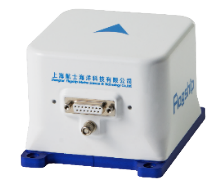
\includegraphics[height=6.5cm]{imagens/MRU1.png}}
                \label{fig:mru1}
            }\hspace{1cm}
            \subfloat[MRU19B]{
                \frame{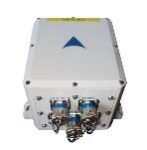
\includegraphics[height=6.5cm]{imagens/MRU2.png}}
                \label{fig:mru2}
            }

            \textbf{Fonte:} \href{http://en.flag-ship.cn/}{http://en.flag-ship.cn/}
            \label{fig:enter-label}
        \end{figure}

        Para maior precisão, os MRUs aplicam filtros digitais, como o de Kalman, que combinam os dados dos sensores para reduzir ruídos e minimizar erros acumulados. Essas medições são essenciais para corrigir oscilações e garantir a estabilidade em operações críticas no ambiente marítimo. Neste estudo, foram consideradas as principais características técnicas que permitem a seleção do dispositivo mais adequado para servir como referência e padrão nas futuras implementações. 
        
        Os quatro melhores MRUs foram selecionados com base nesses critérios e estão apresentados na \autoref{tab:melhores_mrus}. Dentre as especificações escolhidas, destaca-se a faixa angular, que indica a amplitude de ângulos que cada dispositivo pode medir, e a precisão estática em roll e pitch, que avalia a exatidão das medições de inclinação em condições estáticas. Além disso, é analisada a precisão dinâmica para ângulos de até $5^\circ$, essencial para operações em movimento. A proteção contra água e poeira é especificada pela classificação IP.

        \begin{table}[H]
            \centering
            \caption{\small Comparação de MRUs}
            \label{tab:melhores_mrus}
            \vspace{-0.3cm}
            
            \scriptsize
            {\renewcommand{\arraystretch}{2.2}
            \begin{longtable}{|c|c|c|c|c|}
            \hline
                \fcol{4}{\textbf{Especificação}} & 
                \col{2.2}{\textbf{Guidance Marine IMU}} & 
                \col{2.2}{\textbf{InertialLabs MRU-E}} &
                \col{2.2}{\textbf{SBG Ellipse Series}} & 
                \col{2.2}{\textbf{Kongsberg MRU H}} \\
            \hline
                \textbf{Faixa Angular} & $\pm 30^\circ$ & $\pm 90^\circ, \pm 180^\circ$ & 360$^\circ$ & $\pm 180^\circ$ \\
            \hline
                \textbf{Precisão Estática Roll \& Pitch} & 0.02$^\circ$ RMS & 0.03$^\circ$ RMS & $\pm 0.05^\circ$ RMS & 0.03$^\circ$ RMS \\
            \hline
                \textbf{Precisão Dinâmica ($\pm 5^\circ$)} & 0.03$^\circ$ RMS & 0.06$^\circ$ RMS & 0.12$^\circ$ RMS & 0.010$^\circ$ 1-sigma \\
            \hline
                \textbf{Proteção (IP)} & IP67 & IP66 & IP66 & IP66 \\
            \hline
                \textbf{Peso} & 2 kg & 280 g & 45 g & 2.2 kg \\
            \hline
                \textbf{Saída de Dados} & NMEA0183 & RS-422, RS-232 & RS-232, RS-422 & Ethernet, RS-232 \\
            \hline
                \textbf{Ruído Angular (Giroscópio)} & N/A & 0.004$^\circ$/s & 0.0035$^\circ$/s & 0.015$^\circ$/s RMS \\
            \hline
                \textbf{Ruído Acelerômetro} & 0.01 m/s² RMS & 0.025 mg & 0.14 mg/$\sqrt{\text{Hz}}$ & 0.002 m/s² RMS \\
            \hline
                \textbf{Material} & Alumínio Anodizado & Anodizado & Alumínio Anodizado & Anodizado \\
            \hline
                \textbf{Fonte} 
                & \href{https://tinyurl.com/2c8szncn}{\textbf{Ship Motion Control}} 
                &  \href{https://tinyurl.com/2ynmt9mz}{\textbf{Inertial Labs}}
                &  \href{https://tinyurl.com/2ajzynsp}{\textbf{SBG Systems}}
                &  \href{https://tinyurl.com/2xuhy76v}{\textbf{Kongsberg}}\\
                \hline
            \end{longtable}}
    
            \small
            \textbf{Fonte:} \href{https://tinyurl.com/2a54wjmx}{Autoria Própria}
        \end{table}
        \vspace{-0.2cm}
    
        Outros aspectos considerados incluem o peso dos dispositivos e os protocolos de saída de dados, como NMEA0183, RS-232, RS-422 e Ethernet, que garantem a compatibilidade com diferentes sistemas. Em relação ao desempenho, a tabela avalia o ruído angular do giroscópio (em graus por segundo) e o ruído do acelerômetro (em m/s² ou mg), que refletem a precisão das medições. Por fim, destaca-se o material de construção, predominantemente alumínio anodizado, que confere resistência e durabilidade aos dispositivos.
        
        \newpage
        \subsection{Módulos IMU}
            Os IMUs (Unidades de Medição Inercial) são módulos que integram acelerômetros, giroscópios e, em alguns casos, magnetômetros para medir aceleração linear, velocidade angular e orientação no espaço \hyperlink{EMBARCADOS}{(EMBARCADOS, 2019)}. Os acelerômetros detectam mudanças de velocidade nos três eixos, enquanto os giroscópios medem a taxa de rotação. Quando presentes, os magnetômetros ajudam a corrigir desvios na orientação usando o campo magnético terrestre. Assim como os MRUs, os IMUs também processam esses dados por meio de filtros dedicados, garantindo medições mais precisas ao minimizar ruídos e erros acumulados. Eles são amplamente utilizados em navegação, estabilização de plataformas e controle de movimentos em sistemas embarcados e aplicações offshore.

            \begin{figure}[H]
                \centering
                \caption{VN-300 DUAL GNSS/INS}
                \frame{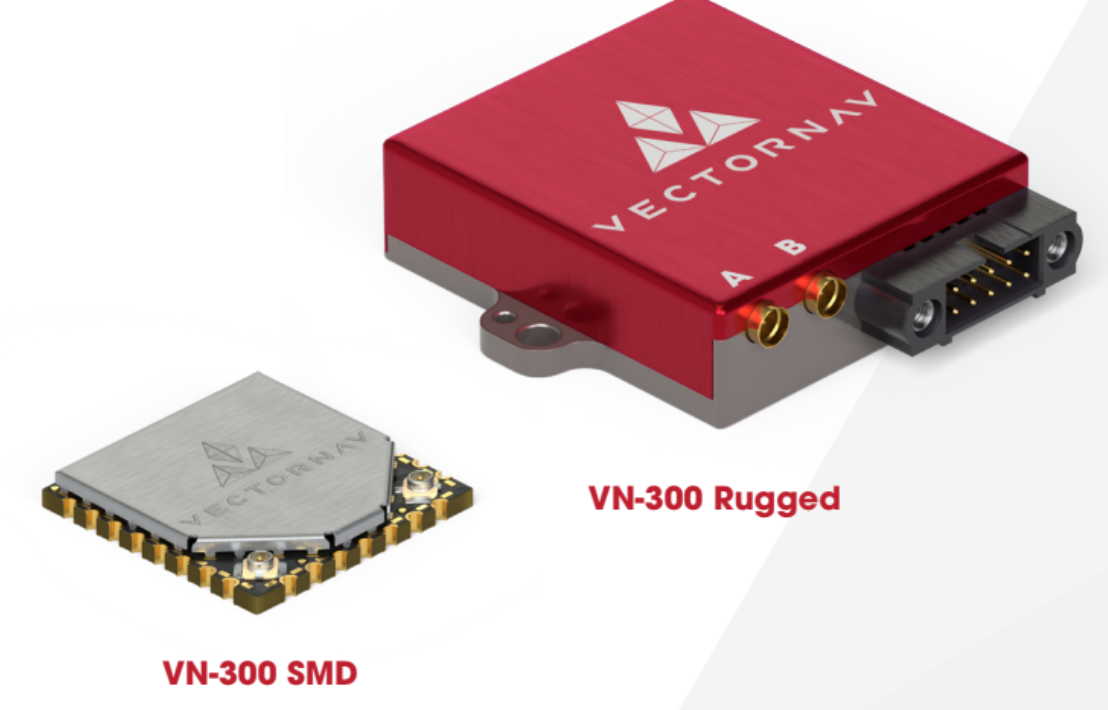
\includegraphics[width=12.5cm]{imagens/vectornav.png}}
    
                \textbf{Fonte:} \href{https://drive.google.com/file/d/10F2b27qL_zZyZodPNqSl0tJQ57hC9PcW/view?usp=sharing}{Vectornav}
                \label{fig:vector}
            \end{figure}

            A \autoref{fig:vector} apresenta o dispositivo VN-300 DUAL GNSS/INS, um sistema de navegação inercial (INS) de alto desempenho, auxiliado por um Sistema Global de Navegação por Satélite (Global Navigation Satellite System - GNSS) e equipado com uma bússola integrada. O dispositivo combina sensores inerciais baseados em MEMS, dois receptores GNSS de alta sensibilidade e algoritmos avançados de filtragem de Kalman, proporcionando estimativas precisas de posição, velocidade e atitude. Embora esses dispositivos possuam um custo mais elevado, sua aquisição é justificada pela alta confiabilidade e robustez, sendo amplamente testados e validados no mercado. Essa característica reduz significativamente o tempo necessário para o desenvolvimento do projeto, permitindo que o foco seja direcionado à implementação do software de monitoramento, uma vez que o sensor utilizado já oferece precisão e eficiência comprovadas.

            \begin{table}[H]
                \centering
                \addtocounter{table}{-1}
                \caption{\small Comparação de 4 Sensores Inerciais com Preço Informado}
                \label{tab:comparacao_4_sensores_preco}
                \vspace{-0.4cm}
                
                \scriptsize
                {\renewcommand{\arraystretch}{2.0}
                \begin{longtable}{|c|c|c|c|c|}
                \hline
                    % Cabeçalho da tabela
                    \fcol{4}{\textbf{Especificação}} & 
                    \col{2.8}{\textbf{IMX-5 (InertialSense)}} &
                    \col{2.8}{\textbf{ADIS16488A (Analog Devices)}} &
                    \col{2.8}{\textbf{ADIS16495-2 (Analog Devices)}} &
                    \col{2.8}{\textbf{MTi-G-710 (Xsens)}} \\
                \hline
                    % Tecnologia
                    \fcol{4}{Tecnologia} & 
                    \col{2.8}{MEMS} &
                    \col{2.8}{MEMS} &
                    \col{2.8}{MEMS} &
                    \col{2.8}{MEMS} \\
                \hline
                    % Faixa Giro
                    \fcol{4}{Faixa de Giro (\(^{\circ}/s\))} & 
                    \col{2.8}{\(\pm 4000\)} &
                    \col{2.8}{\(\pm 450\)} &
                    \col{2.8}{\(\pm 450\) a \(\pm 480\)} &
                    \col{2.8}{\(\pm 450\)} \\
                \hline
                    % Faixa Aceleração
                    \fcol{4}{Faixa de Aceleração (g)} & 
                    \col{2.8}{\(\pm 16\)} &
                    \col{2.8}{\(\pm 18\)} &
                    \col{2.8}{\(\pm 8\)} &
                    \col{2.8}{\(\pm 16\)} \\
                \hline
                    % Taxa máxima de saída
                    \fcol{4}{Taxa Máxima de Saída} & 
                    \col{2.8}{1000\,Hz (IMU), 200\,Hz (AHRS)} &
                    \col{2.8}{2.4\,kHz} &
                    \col{2.8}{4.25\,kHz} &
                    \col{2.8}{Até 2000\,Hz} \\
                \hline
                    % Tensão de Alimentação
                    \fcol{4}{Tensão de Alimentação} & 
                    \col{2.8}{4.5--20\,V} &
                    \col{2.8}{3.0--3.6\,V} &
                    \col{2.8}{3.0--3.6\,V} &
                    \col{2.8}{3.3 ou 4.5--34\,V} \\
                \hline
                    % Interface
                    \fcol{4}{Interface} & 
                    \col{2.8}{USB, UART, RS232,\\ RS485, CAN, SPI} &
                    \col{2.8}{SPI} &
                    \col{2.8}{SPI} &
                    \col{2.8}{USB, RS232, RS422,\\ UART} \\
                \hline
                    % Dimensões
                    \fcol{4}{Dimensões (mm)} & 
                    \col{2.8}{30.5\,\(\times\)\,25.4\,\(\times\)\,14.8} &
                    \col{2.8}{47\,\(\times\)\,44\,\(\times\)\,14} &
                    \col{2.8}{47\,\(\times\)\,44\,\(\times\)\,14} &
                    \col{2.8}{57\,\(\times\)\,41.9\,\(\times\)\,23.6} \\
                \hline
                    % Peso
                    \fcol{4}{Peso (g)} & 
                    \col{2.8}{14} &
                    \col{2.8}{48} &
                    \col{2.8}{42} &
                    \col{2.8}{58} \\
                \hline
                    % Faixa de Preço
                    \fcol{4}{Faixa de Preço (USD)} & 
                    \col{2.8}{\$3999} &
                    \col{2.8}{\$2.713,83} &
                    \col{2.8}{\$3.891,46} &
                    \col{2.8}{\$\;5.379,00} \\
                \hline
                    % Faixa de Preço
                        \fcol{4}{Fonte} & 
                        \col{2.8}{\href{https://tinyurl.com/26ql2oyc}{\textbf{Inertial Sense}}} &
                        \col{2.8}{\href{https://tinyurl.com/29t2k9k3}{\textbf{Analog Devices}}} &
                        \col{2.8}{\href{https://tinyurl.com/22vfo3vz}{\textbf{Analog Devices}}} &
                        \col{2.8}{\href{https://tinyurl.com/28yen2rh}{\textbf{Movella}}} \\
                    \hline
                \end{longtable}}
                
                \small
                \textbf{Fonte:} \href{https://tinyurl.com/2a54wjmx}{Autoria Própria}
            \end{table}
        
            A \autoref{tab:comparacao_4_sensores_preco} apresenta a comparação entre os IHMs selecionados como os mais adequados para o projeto, considerando dispositivos com comportamentos similares e que atendem aos critérios essenciais de precisão e confiabilidade. Tais dispositivos foram escolhidos por alinharem-se ao escopo do projeto, oferecendo uma solução tecnicamente viável e financeiramente vantajosa. Em comparação com os MRUs, que possuem um custo elevado e menor possibilidade de parametrização, os IHMs selecionados proporcionam maior flexibilidade no desenvolvimento, facilitando a implementação de novas funcionalidades e aprimoramentos conforme as necessidades do sistema.
            
    
        
        \newpage
        \subsection{Módulos Sensoriais}
            Assim como as Unidades de Medida Inercial (IMUs), os módulos de sensores que incorporam acelerômetros e giroscópios operam com base no mesmo princípio de medição. No entanto, esses módulos apresentam vantagens em termos de custo reduzido, compactação e integração de funcionalidades de filtragem e processamento diretamente no próprio sensor \hyperlink{MORAES}{(MORAES, 2015)}. Essa característica proporciona maior autonomia no desenvolvimento, permitindo maior flexibilidade na personalização e parametrização do dispositivo, de acordo com os requisitos específicos do projeto. A figura \ref{fig:IMUHWT} se refere a um módulo pesquisado com filtros embutidos e alta precisão de operação.
        
        \begin{figure}[H]
            \centering
            \caption{Giroscópio HWT901B}
            \frame{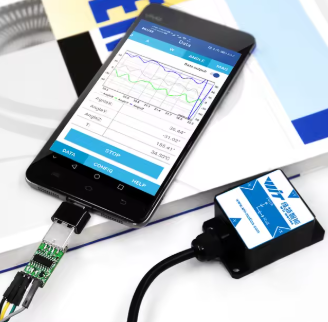
\includegraphics[width=10cm]{imagens/IMU1.png}}

            \textbf{Fonte:} \href{https://pt.aliexpress.com/item/1005003003878184.html?src=google&p4pItemId=1005003003878184&p4pAdGroupId=5000366617792&isp4p=y&src=google&albch=shopping&acnt=768-202-3196&isdl=y&slnk=&plac=&mtctp=&albbt=Google_7_shopping&aff_platform=google&aff_short_key=UneMJZVf&gclsrc=aw.ds&&albagn=888888&&ds_e_adid=&ds_e_matchtype=&ds_e_device=c&ds_e_network=x&ds_e_product_group_id=&ds_e_product_id=pt1005003003878184&ds_e_product_merchant_id=5504851841&ds_e_product_country=BR&ds_e_product_language=pt&ds_e_product_channel=online&ds_e_product_store_id=&ds_url_v=2&albcp=21441683223&albag=&isSmbAutoCall=false&needSmbHouyi=false&gad_source=1&gclid=CjwKCAiAh6y9BhBREiwApBLHC7Kg5nlv6oe2giDEG37Kpom1dDxg_jnecd6Po3CKCnHOabN7uA81WBoCKqwQAvD_BwE}{AliExpress}
            \label{fig:IMUHWT}
        \end{figure}        

        Os sensores serão utilizados em testes de bancada conduzidos pela equipe de desenvolvimento. A medição da aceleração e inclinação em tempo real será realizada por meio de acelerômetros e giroscópios integrados a módulos responsáveis pelo sensoriamento e processamento dos dados. Esses módulos incorporam técnicas de filtragem e comunicação por protocolos específicos, proporcionando maior precisão em comparação à leitura analógica direta. Diante disso, os principais sensores foram analisados, e suas características estão detalhadas na tabela comparativa.
    
        \begin{table}[H]
            \centering
            \addtocounter{table}{-1}
            \caption{\small Comparação de Sensores Acelerômetros/Giroscópios}
            \label{tab:comparacao_sensores}
            \vspace{-0.4cm}
            
            \scriptsize
            {\renewcommand{\arraystretch}{1.5}
            \begin{longtable}{|c|c|c|c|c|}
            \hline
                \fcol{4}{\textbf{Especificação}} & 
                \col{2.6}{\textbf{HWT9053-485}} & 
                \col{2.6}{\textbf{WTGAHRS3}} &
                \col{2.6}{\textbf{HWT901B}} & 
                \col{2.6}{\textbf{MPU-6050}} \\
            \hline
                \fcol{4}{Precisão Angular} & 
                \col{2.6}{$\pm 0.001^\circ$} & 
                \col{2.6}{$0.05^\circ$ (estático), $0.1^\circ$ (dinâmico)} & 
                \col{2.6}{$0.05^\circ$} & 
                \col{2.6}{$\pm 0.05^\circ$} \\
            \hline
                \fcol{4}{Interface} & 
                \col{2.6}{RS485 Modbus} & 
                \col{2.6}{TTL/RS232/485} & 
                \col{2.6}{TTL/RS232/485} & 
                \col{2.6}{I²C, SPI} \\
            \hline
                \fcol{4}{Tensão de Alimentação} & 
                \col{2.6}{5-36V} & 
                \col{2.6}{5-36V} & 
                \col{2.6}{3.3-5V (TTL), 9-36V (RS232/RS485)} & 
                \col{2.6}{2.375V-3.46V} \\
            \hline
                \fcol{4}{Frequência Máxima de Saída} & 
                \col{2.6}{921600 baud} & 
                \col{2.6}{200Hz} & 
                \col{2.6}{200Hz} & 
                \col{2.6}{1kHz} \\
            \hline
                \fcol{4}{Resistência à Água} & 
                \col{2.6}{IP67} & 
                \col{2.6}{IP67} & 
                \col{2.6}{Não especificado} & 
                \col{2.6}{Não especificado} \\
            \hline
                \fcol{4}{Chip Principal} & 
                \col{2.6}{ADXL355 + MMC3630} & 
                \col{2.6}{ICM4260X} & 
                \col{2.6}{RM3100} & 
                \col{2.6}{MPU-6050} \\
            \hline
                \fcol{4}{Peso} & 
                \col{2.6}{Sensor: 52.8g, Cabo: 43.7g} & 
                \col{2.6}{Não especificado} & 
                \col{2.6}{Não especificado} & 
                \col{2.6}{4x4x0.9mm (QFN)} \\
            \hline
                \fcol{4}{Saída de Dados} & 
                \col{2.6}{aceleração e inclinação} & 
                \col{2.6}{aceleração, inclinação, latitude e longitude} & 
                \col{2.6}{aceleração, ângulo e taxa angular} & 
                \col{2.6}{aceleração e inclinação} \\
            \hline
                \fcol{4}{Consumo de Corrente} & 
                \col{2.6}{Não especificado} & 
                \col{2.6}{$<$40mA} & 
                \col{2.6}{40mA típico} & 
                \col{2.6}{3.9mA (com DMP)} \\
            \hline
                \fcol{4}{Faixa de Temperatura} & 
                \col{2.6}{-40 a +85 ºC} & 
                \col{2.6}{-40 a +85 ºC} & 
                \col{2.6}{-40 a +85 ºC} & 
                \col{2.6}{-40 a +85 ºC} \\
            \hline
                \fcol{4}{Link} & 
                \col{2.6}{\href{https://tinyurl.com/27jjdfro}{\textbf{AliExpress}}} & 
                \col{2.6}{\href{https://tinyurl.com/28zhbses}{\textbf{AliExpress}}} & 
                \col{2.6}{\href{https://tinyurl.com/25qoo7x6}{\textbf{Fonte}}} & 
                \col{2.6}{\href{https://tinyurl.com/2bxgc9ue}{\textbf{RoboCore}}} \\
            \hline
            \end{longtable}}
            
            \small
            \textbf{Fonte:} \href{https://tinyurl.com/2a54wjmx}{Autoria Própria}
        \end{table}
        \vspace{-0.2cm}
            
        Os dispositivos serão adquiridos a fim de avaliar a precisão e a confiabilidade do sistema. Com base nessas análises, será desenvolvido um software de monitoramento, que será implementado em um microprocessador para viabilizar a aquisição e o processamento dos dados, permitindo a apresentação das informações. O microprocessador deverá contar com um circuito dedicado, integrado aos sensores, possibilitando a fabricação de uma placa de circuito impresso específica para o projeto. Além disso, fatores ambientais, como temperatura e umidade, devem ser considerados, uma vez que o encapsulamento do sistema deverá garantir resistência a testes de submersão e exposição a altas temperaturas.


    \newpage
    \subsection{Definição da Solução Técnica}
        O produto final do projeto será um Dispositivo de Referência de Monitoramento dos Movimentos (DRMM), um MRU (Motion Reference Unit) nacional desenvolvido especificamente para aplicações em helidecks e guindastes offshore. 

        \subsubsection{Requisitos}
            Dentre os principais requisitos de aceitação do projeto pelo cliente no que se refere ao dispositivo, o produto final deve conter: 
    
            \begin{enumerate}
                \item Sensores de última geração, incluindo acelerômetros e giroscópios de alta precisão.
                \vspace{-0.15cm}
                
                \item Firmware customizado, com algoritmos de filtragem de ruído e fusão sensorial.
                \vspace{-0.15cm}
                
                \item Software de comunicação avançado, permitindo integração com sistemas supervisórios offshore.
                \vspace{-0.15cm}
                
                \item Calibragem automatizada, garantindo medições confiáveis ao longo do tempo.
                \vspace{-0.15cm}
                
                \item Design modular e escalável, facilitando futuras atualizações e adaptações para diferentes aplicações offshore.
            \end{enumerate}
            \vspace{-0.1cm}

        
        O projeto inclui um sistema de indicação de dados ao usuário, assegurando que as informações coletadas pelos sensores sejam processadas e apresentadas de forma acessível para supervisão e tomada de decisões. A pesquisa realizada pela \textbf{SMC MRU Motion Lab} \hyperlink{SHIPMOTION}{(SHIPMOTION, 2023)} possibilitou uma compreensão mais aprofundada sobre a estruturação desse sistema. 
        
        \begin{figure}[H]
            \centering
            \caption{Sistema Exemplo de Monitoramento de Inclinação}
            \frame{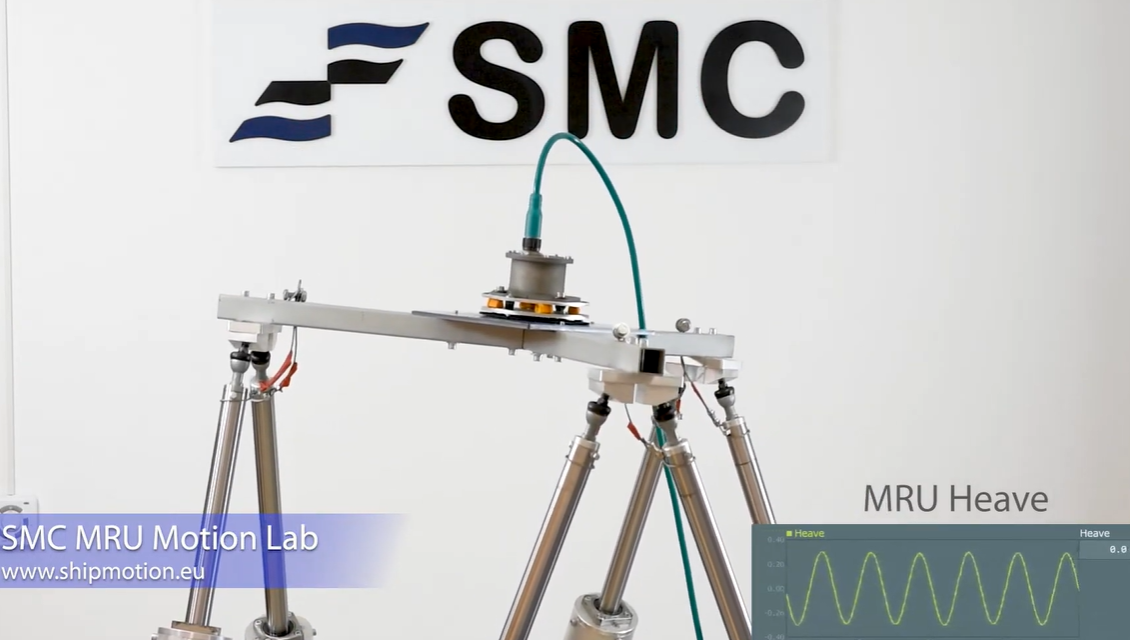
\includegraphics[width=13.5cm]{imagens/SIST.png}}

            \textbf{Fonte:} \href{https://www.youtube.com/watch?v=FVuUqbL0Rb0}{SMC MRU Motion Lab}
            \label{fig:youtube}
        \end{figure}
        \vspace{-0.1cm}
        
        Conforme ilustrado na \autoref{fig:youtube}, é possível observar um sistema de monitoramento gráfico do dispositivo, no qual uma superfície é inclinada por atuadores em um movimento senoidal, exibindo graficamente a posição vertical do ponto focal, representado pelo sensor. Esse sistema poderá ser aprimorado por meio do desenvolvimento de um software dedicado, sendo necessário definir a abordagem mais adequada para sua implementação.

        Com intuito de obter maior compreensão acerca das variáveis de estudo, a equipe projetou circuito base de como funcionaria o sistema utilizando o sensor MPU6050, que constitui um acelerômetro e um giroscópio conectados em um Arduino que por comunicação I2C \hyperlink{ELECTRONOOBS}{(ELECTRONOOBS, 2018)}, recebe dados de aceleração e inclinação no tempo e os envia para um microprocessador Raspberry PI, que aplica um filtro de Kalman Simples nos dados de aceleração para filtrá-los e convertê-los para posição e velocidade. A figura subsequente mostra a implementação feita para fins de teste.
        
        \vspace{.3cm}
        \begin{figure}[H]
            \centering
            \caption{Prototipagem de um Circuito Simples de Acelerômetro}

            \subfloat[Componentes]{
                \frame{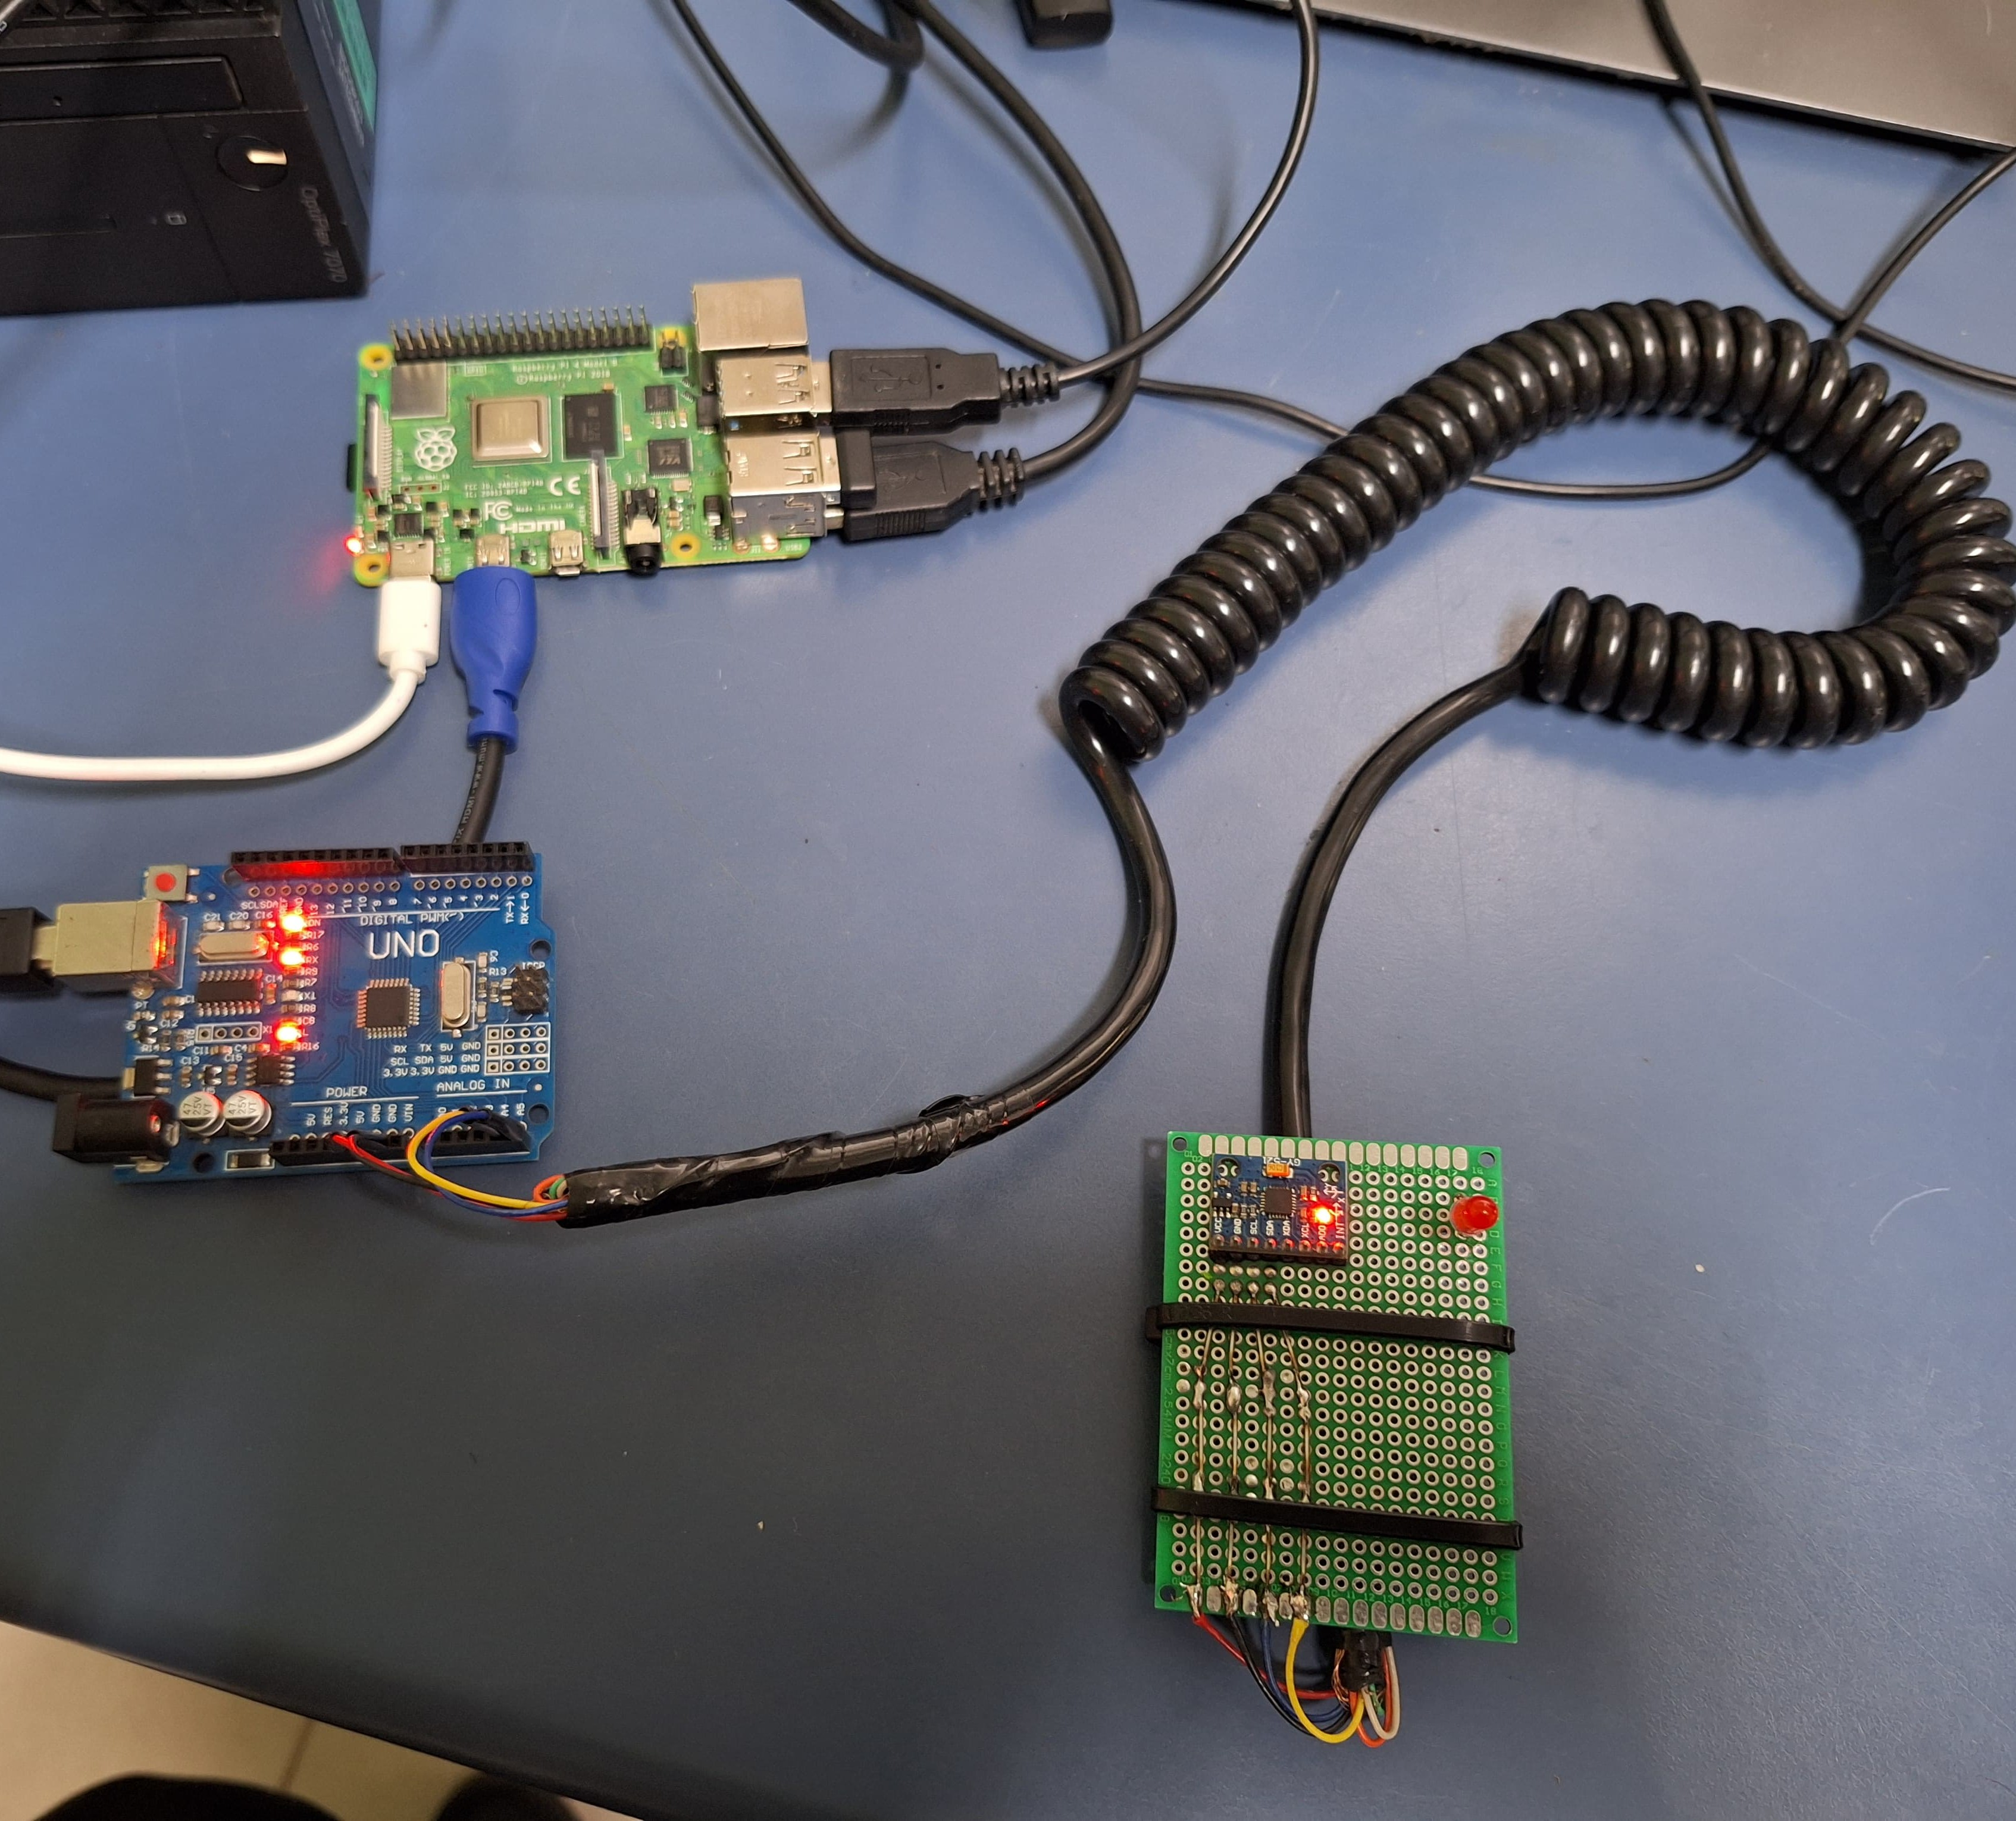
\includegraphics[height=7.7cm]{imagens/prot2.jpeg}}
            }\hfill
            \subfloat[Simulação]{
                \frame{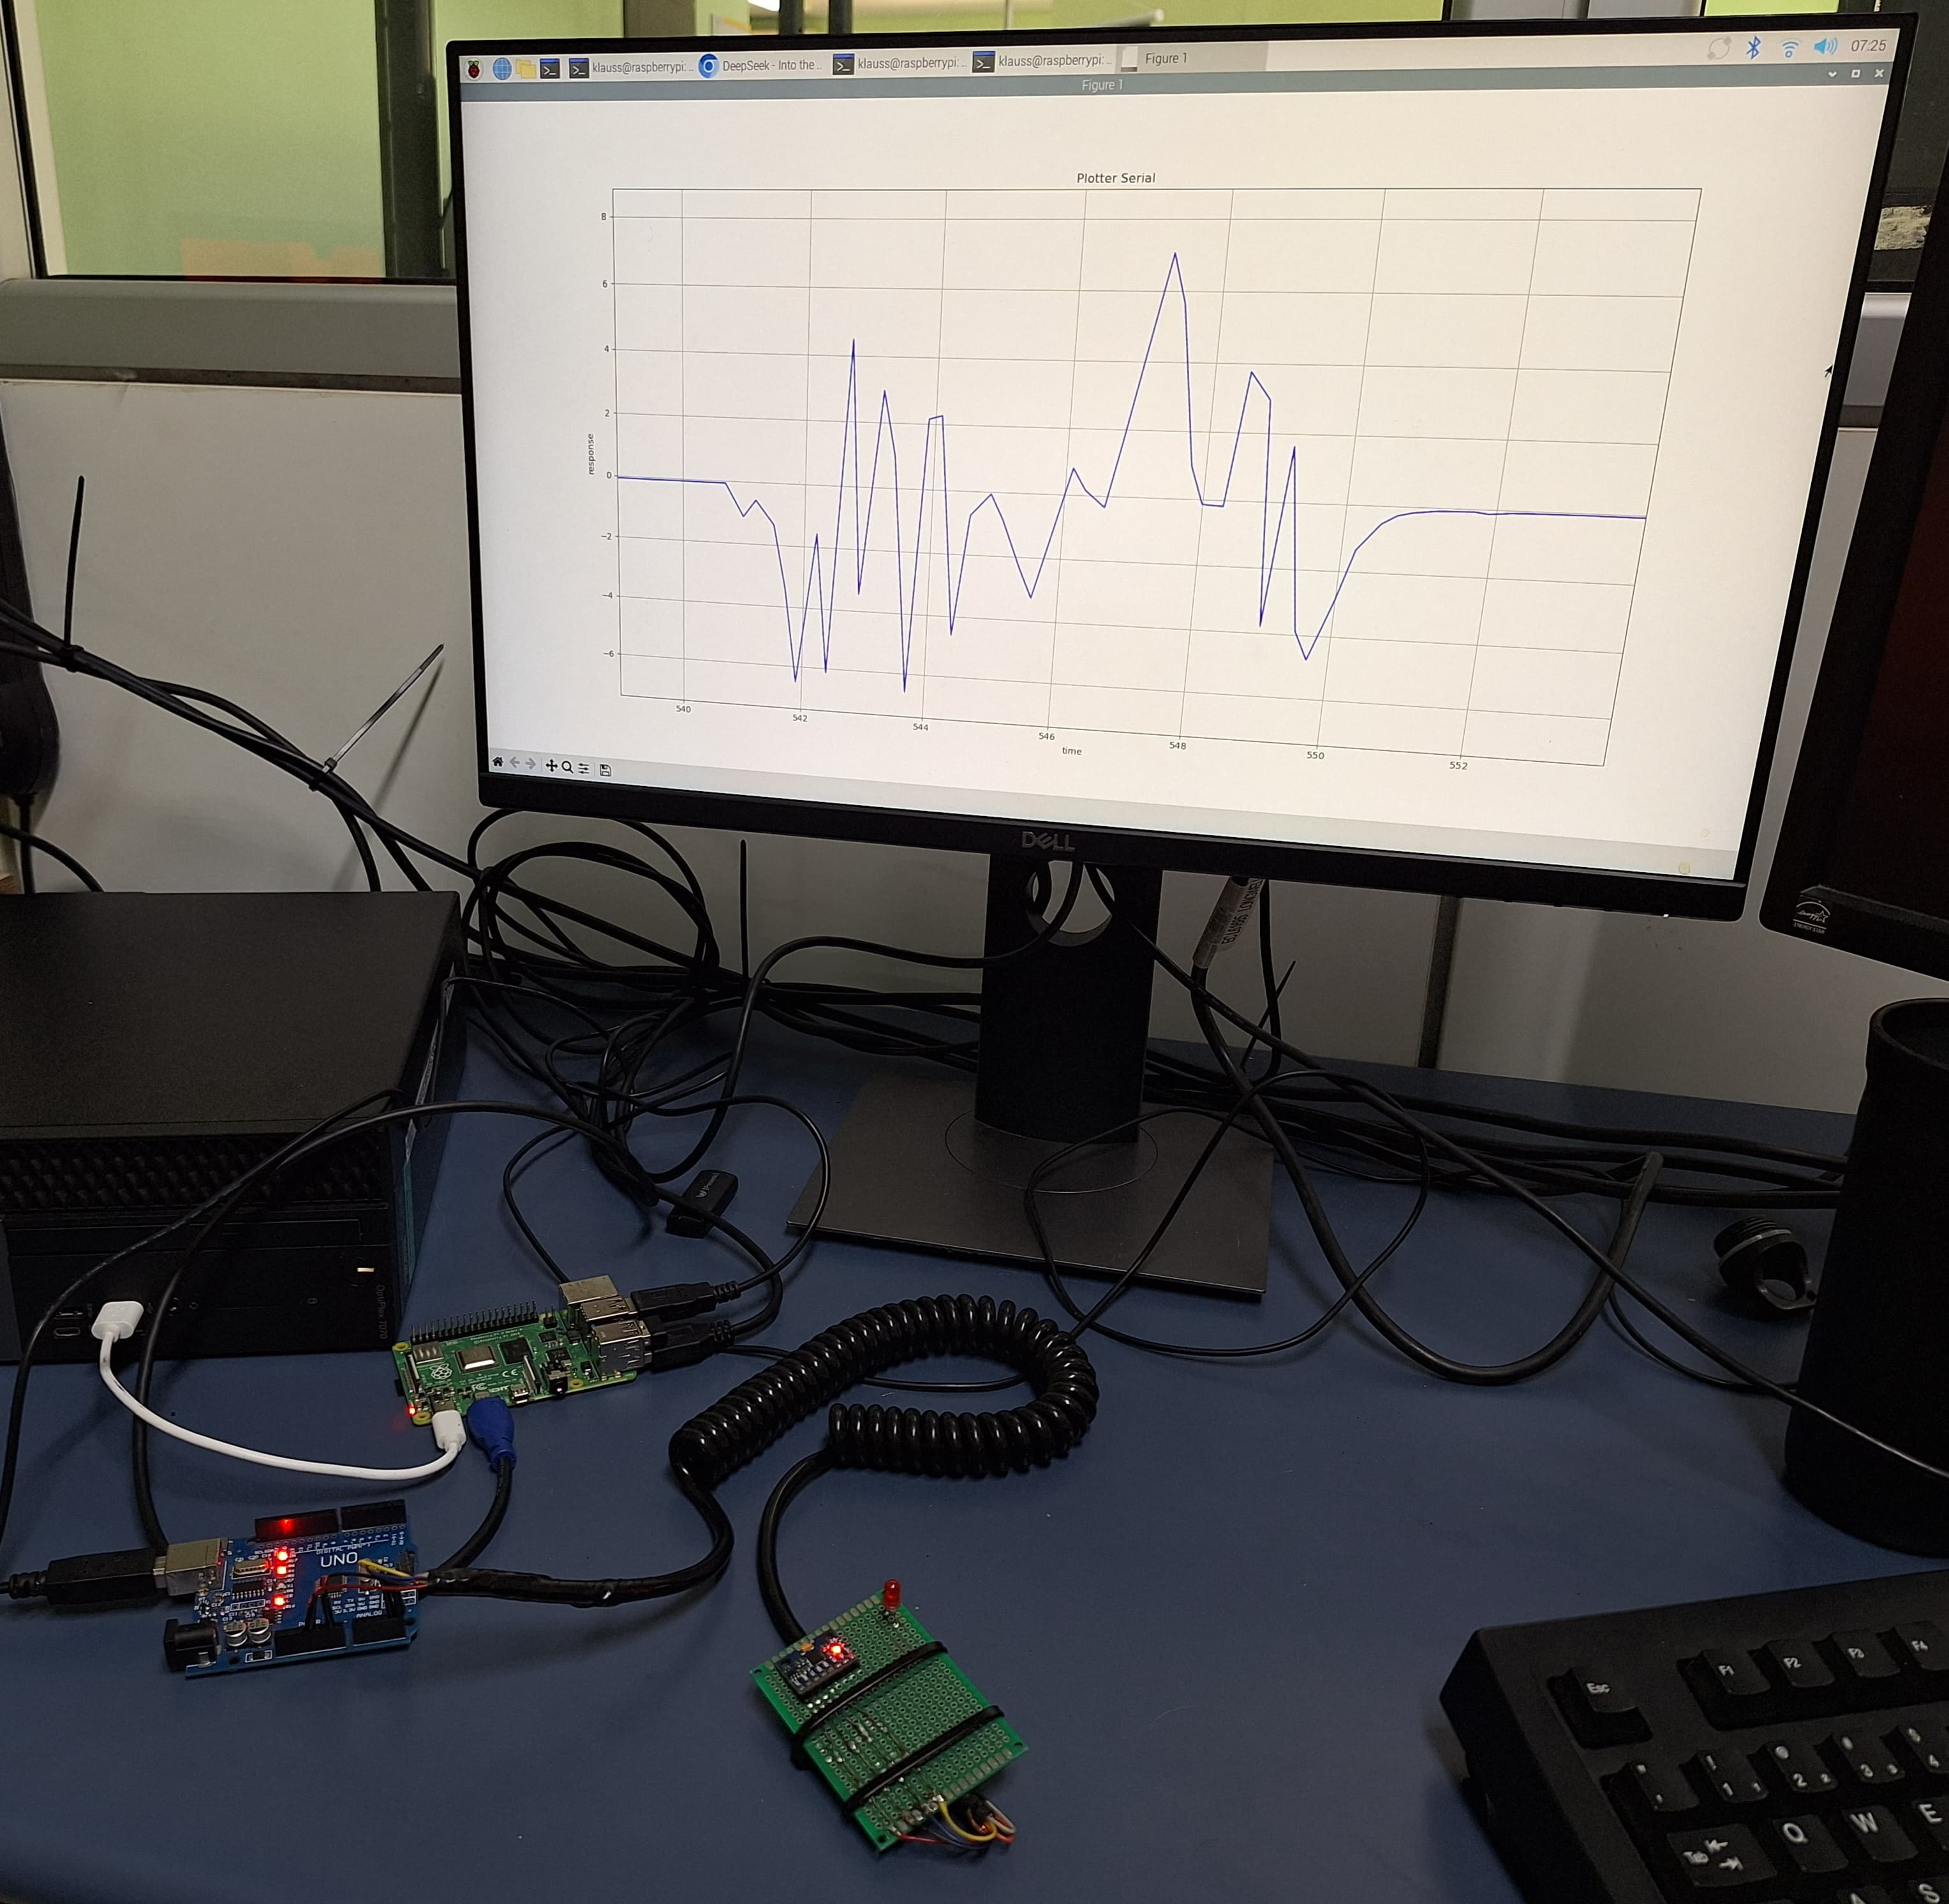
\includegraphics[height=7.7cm]{imagens/prot1.jpeg}}
            }

            \vspace{.3cm}
            \textbf{Fonte:} Autoria Própria
            \label{fig:prot}
        \end{figure}
        
        Existem diversas formas de alcançar uma solução técnica satisfatória, e cada uma traz riscos específicos. A aquisição de módulos MRU prontos no mercado, por exemplo, simplificaria o processo ao exigir apenas a criação de uma interface e a comunicação com o microprocessador. Ainda assim, essa via pode se tornar inviável financeiramente, seja pelo alto custo, seja pela falta de retorno econômico.
        
        Em contrapartida, construir um MRU a partir de sensores individuais implica desenvolver algoritmos para filtrar os dados, integrar diferentes sensores, projetar o encapsulamento e realizar testes de robustez. Mesmo assim, há o risco de não se atingir a precisão esperada, além de demandar um longo período para homologação e patenteamento. A \autoref{tab:compdevices} mostra uma comparação entre os diferentes dispositivos com base em suas vantagens e desvantagens de mercado.

        \begin{table}[H]
            \centering
            \addtocounter{table}{-1}
            \caption{\small Comparação de Dispositivos de Mercado}
            \label{tab:compdevices}
            \vspace{-0.4cm}
            
            \scriptsize
            {\renewcommand{\arraystretch}{2.0}
            \begin{longtable}{|c|c|c|c|}
            \hline
                \fcol{4}{\textbf{Critério}} & 
                \col{2.6}{\textbf{MRUs}} & 
                \col{2.6}{\textbf{IMUs}} &
                \col{3.2}{\textbf{Módulos Sensoriais}} \\
            \hline
                \fcol{4}{Precisão} & 
                \col{2.6}{Alta} & 
                \col{2.6}{Média} &
                \col{3.2}{Baixa a Média} \\
            \hline
                \fcol{4}{Custo} & 
                \col{2.6}{Alto} & 
                \col{2.6}{Médio} &
                \col{3.2}{Baixo} \\
            \hline
                \fcol{4}{Nível de Parametrização} & 
                \col{2.6}{Baixo} & 
                \col{2.6}{Médio} &
                \col{3.2}{Alto} \\
            \hline
                \fcol{4}{Facilidade de Integração} & 
                \col{2.6}{Média} & 
                \col{2.6}{Média} &
                \col{3.2}{Alta (exige maior esforço de desenvolvimento)} \\
            \hline
                \fcol{4}{Robustez} & 
                \col{2.6}{Alta} & 
                \col{2.6}{Média} &
                \col{3.2}{Baixa a Média} \\
            \hline
                \fcol{4}{Durabilidade} & 
                \col{2.6}{Alta} & 
                \col{2.6}{Média} &
                \col{3.2}{Baixa a Média} \\
            \hline
                \fcol{4}{Compatibilidade} & 
                \col{2.6}{Sim (protocolos marítimos e industriais)} & 
                \col{2.6}{Sim (dependendo do modelo)} &
                \col{3.2}{Não (exige "bridge"\ ou firmware custom)} \\
            \hline
            \end{longtable}}

            \vspace{.15cm}
            \small
            \textbf{Fonte:} Autoria Própria
        \end{table}
        \vspace{-0.2cm}


         Apesar da alta precisão dos MRUs, a facilidade de integração e parametrização são relativamente baixas, o que impede autonomia da equipe para manutenção e desenvolvimento de novas funcionalidades. Entretanto, o estudo e pesquisa permitirão desvendar se é possível aumentar a precisão a partir de sensores menos potentes através de algoritmos avançados como redes neurais ou ajuste de funções multivariáveis. Assim sendo, para otimizar o projeto e evitar desperdiçar recursos em alternativas que podem não funcionar, decidiu-se dividir o trabalho em três equipes autônomas, cada uma focada em uma dessas abordagens.
    
        \vspace{.15cm}
        \subsubsection{Equipe 1}
            A primeira equipe deverá adquirir os módulos de acelerômetros e giroscópios, compreendendo seu funcionamento e protocolo de comunicação. Caso necessário, será conduzido um estudo sobre técnicas de filtragem de dados, como filtros de frequência e o filtro de Kalman, para assegurar a precisão das medições. Os dados serão exibidos em tempo real nas coordenadas x, y e z, permitindo a visualização da posição atual por meio de software dedicado. Para viabilizar o processamento das informações, será realizada a pesquisa e seleção de um processador adequado, considerando sua capacidade de executar operações matemáticas com eficiência. Além disso, fatores ambientais, como o aquecimento do compartimento onde o DRMM será instalado, deverão ser analisados para prevenir superaquecimento e garantir a resistência do sistema, essencial para a realização dos testes de submersão.

        \vspace{.15cm}
        \subsubsection{Equipe 2}
            A segunda equipe realizará a pesquisa e aquisição de sensores e módulos, como MRUs, que possuam funcionalidades integradas, com dados previamente filtrados e processados, visando otimizar tempo e recursos no desenvolvimento do projeto. Além disso, deverá ser estabelecida a comunicação desses dispositivos com o software de monitoramento desenvolvido em paralelo. Os dados obtidos a partir dos MRUs comerciais servirão como referência para a equipe responsável pelo processamento, permitindo uma comunicação bilateral entre os grupos. Essa abordagem possibilita a implementação de um sistema de contingência, garantindo que, em caso de falha no processamento desenvolvido, os MRUs adquiridos possam ser utilizados como fonte principal de dados, assegurando a continuidade das operações e o aprimoramento das funcionalidades do projeto.

        \vspace{.15cm}
        \subsubsection{Equipe 3}
            A terceira equipe será responsável por identificar e estabelecer os principais protocolos de comunicação utilizados para a integração com os MRUs, garantindo compatibilidade com os desenvolvimentos realizados pelas equipes 1 e 2. O desenvolvimento será conduzido de forma paralela e independente, possibilitando a integração com os módulos selecionados por qualquer uma das equipes. Adicionalmente, essa equipe terá a função de pesquisar e cotar serviços de calibração, além de viabilizar a aquisição de hexapods para a criação de um ambiente adequado para testes e validação do sistema.

        \vspace{.15cm}
        \subsubsection{Esquematização Geral}
            Independentemente da abordagem adotada ao final do projeto, observa-se um padrão geral de estrutura necessário para a construção do dispositivo. Essa estrutura pode ser desenvolvida a partir do estudo de sistemas similares que possuam objetivos equivalentes. Nesse contexto, a \autoref{fig:esquema} ilustra a ideia geral do produto, contemplando processos de comunicação, aquisição e filtragem de dados. Ressalta-se ainda que a sequência ou a ordem dos componentes pode variar, sendo esta disposição apresentada apenas para fins de visualização e compreensão geral dos elementos e de sua integração com diferentes dispositivos e sensores.

            \newpage
            Os sensores constituem a base do sistema e podem ser IMUs integradas ou módulos que reúnam magnetômetros, giroscópios e acelerômetros, com ou sem sistemas de filtragem ou pré-processamento embutidos. Também é possível empregar múltiplos sensores da mesma grandeza para obter redundância e aprimorar a precisão das leituras, permitindo comparações. Além disso, encoders ou conversores digitais podem ser instalados próximos aos sensores para preparar e enviar os dados à camada superior.

            \begin{figure}[H]
                \centering
                \caption{Diagrama Esquemático da Solução Técnica}
                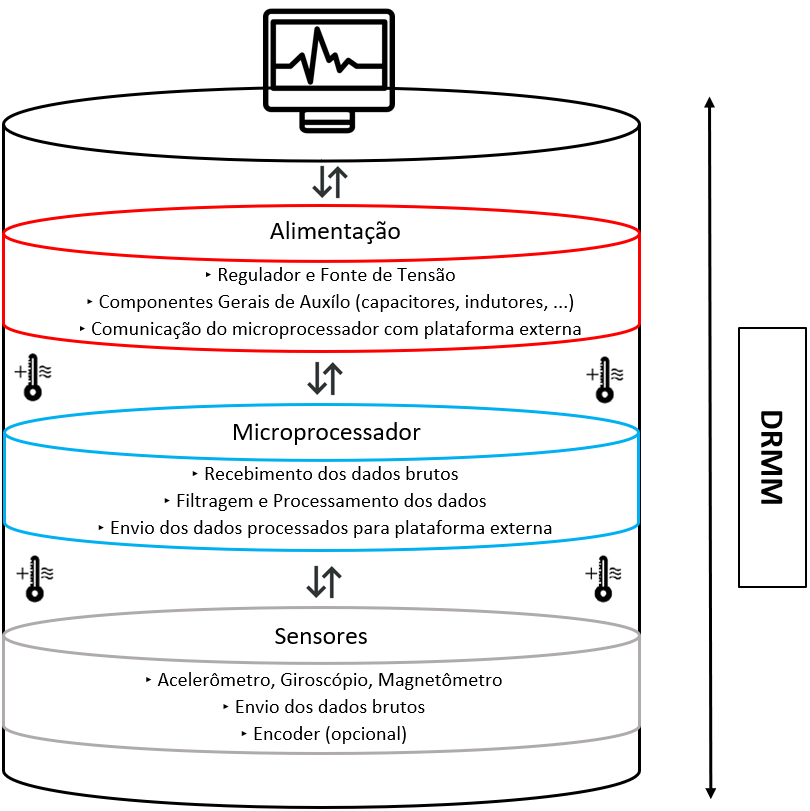
\includegraphics[width=13cm]{imagens/MRU Esquem.png}

                \textbf{Fonte}: Autoria própria
                \label{fig:esquema}
            \end{figure}

            O microprocessador é responsável pelo processamento de dados e pela obtenção de variáveis essenciais para o objetivo do sistema. Ao receber as informações dos sensores, organiza-as e as envia para a plataforma externa (primeira camada). É fundamental considerar o sobreaquecimento do compartimento que abriga os componentes, selecionando um dispositivo com baixa geração de calor e um material de invólucro que proporcione boa dissipação térmica, além de ser resistente e robusto. Assim, evitam-se problemas de superaquecimento e possíveis danos causados por umidade ou líquidos.
        
\newpage
\section{Pesquisa de Atuadores}
    Os atuadores serão utilizados no projeto para a calibração dinâmica do Dispositivo de Referência de Monitoramento dos Movimentos (DRMM), permitindo a simulação controlada de oscilações, inclinações e acelerações. Sua aplicação possibilita a avaliação da resposta dos sensores, o ajuste de parâmetros, a correção de erros e a validação dos algoritmos de fusão de dados, garantindo medições precisas e confiáveis antes da operação em ambientes offshore \hyperlink{UNICAMP}{(UNICAMP, 2021)}.
    

    \subsection{Calibração Externa (Acutronic)}
        Com objetivo de garantir que o produto final atinja o mesmo nível de precisão e confiabilidade dos equipamentos de referência disponíveis no mercado, busca-se validar se o dispositivo é capaz de medir de forma correta roll, pitch e heave (ou demais graus de liberdade), dentro das tolerâncias especificadas, sob condições controladas de rotação, aceleração e temperatura. Esse conjunto permite formular um sistema de calibração que deve possuir requisitos que permitem alcançar as metas estabelecidas.
        
        A \autoref{fig:kong} mostra um sistema de calibração funcional desenvolvido pela empresa Kongsberg. Dessa forma, o estudo destaca justamente o uso de máquinas de calibração de dois eixos com câmara climática integrada (Acutronic) para assegurar que cada MRU saia de fábrica (ou retorne de um serviço de recalibração) dentro das especificações de fábrica.

        \vspace{.3cm}
        \begin{figure}[H]
            \centering
            \caption{Sistema de Calibração da Kongsberg}
            \frame{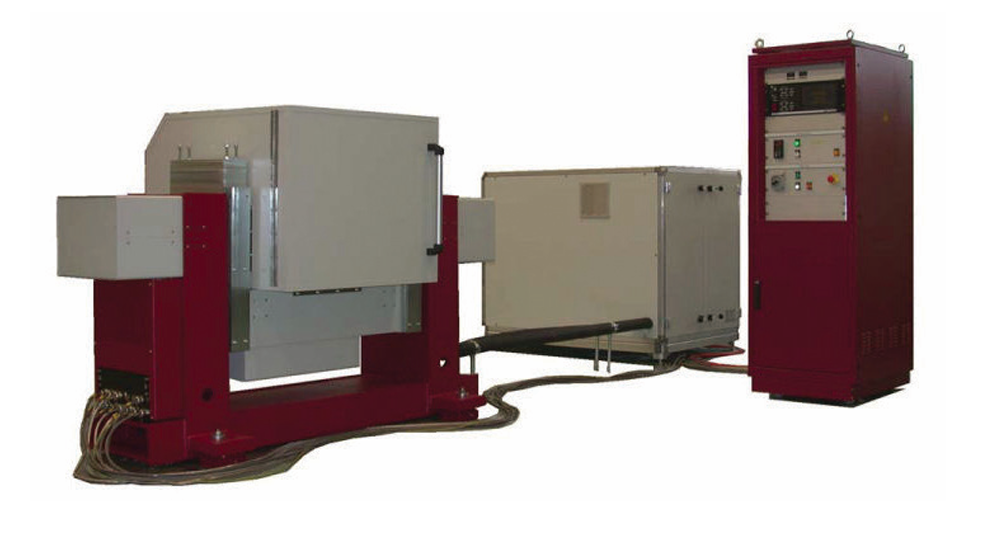
\includegraphics[width=14cm]{imagens/calib.png}}
            
            \textbf{Fonte:} \href{https://drive.google.com/file/d/1SQvDLzpfvZJxshEj6cRBlBmzcynMaB-o/view?usp=sharing}{Kongsberg}
            \label{fig:kong}
        \end{figure}
        \vspace{-0.1cm}

        A Acutronic produz mesas de calibração e ensaio (turntables) de dois ou mais eixos, capazes de posicionar o MRU em diferentes ângulos (roll e pitch, por exemplo) e em variadas velocidades de rotação. O procedimento descrito consiste em colocar o dispositivo em uma mesa de testes Acutronic, aplicar rotações e ciclos de temperatura para medir, ajustar e validar, e, por fim, emitir um certificado de calibração que atesta se o DRMM atende aos limites de erro especificados. Com isso, pode-se criar um roteiro padrão do que deve ser feito para a calibração do dispositivo desenvolvido.

        \begin{enumerate}
            \item O DRMM é fixado na plataforma de teste para que cada eixo de medição (roll, pitch, yaw) seja exercitado de forma precisa.
            
            \item A Acutronic executa rotações controladas e movimentos cíclicos, enquanto sensores de referência internos monitoram a posição e velocidade exatas.
            
            \item Os dados gerados pelo DRMM em teste são comparados aos dados “verdadeiros” (a referência fornecida pela máquina de calibração). Isso permite identificar desvios de escala, offset e possíveis não-linearidades.
            
            \item Com base nessa análise, são aplicados coeficientes de correção (ganhos, offsets, matrizes de alinhamento) no firmware do DRMM para alinhar as medições às condições reais de uso. Esse processo pode ser repetido diversas vezes, até que o erro do equipamento fique dentro das tolerâncias definidas.
            
            \item Ao fim do processo, gera-se um relatório/certificado atestando a acurácia final do dispositivo, a temperatura de teste e a data do ensaio.
        \end{enumerate}

        Um paralelo que pode ser feito com a solução técnica é utilizar este procedimento de calibração para a construção de modelos de inteligência artificial que encontram padrões entre as medições reais e lidas pelo sensor, para aprender e melhorar a precisão dos dados a partir dessa mesma relação. Um exemplo simples seria o uso de aprendizado de máquina ou redes neurais para encontrar uma relação entre a medida dos últimos dados de um ou mais sensores medindo a mesma variável. Assim sendo, o modelo entende o comportamento e pode gerar predições dos dados reais, o que ganha cada vez mais destaque na indústria de tecnologia.
    
    \newpage
    \subsection{Hexapod}
        Os Hexapods são plataformas de movimentação com seis graus de liberdade (6-DOF), permitindo deslocamentos lineares e rotações em torno dos eixos X, Y e Z com alta precisão  \hyperlink{PI}{(PHYSIK INSTRUMENTE, 2025)}. São amplamente utilizados em testes e calibração de sensores, garantindo a replicação controlada de condições dinâmicas reais. No contexto do projeto, seriam utilizados na validação de medições e algoritmos, assegurando a confiabilidade dos dados antes da aplicação em ambientes offshore. A \autoref{fig:hexapod1} mostra um Hexapod conhecido da empresa Physik Instrumente. 

        \begin{figure}[H]
            \centering
            \caption{Hexapod de 6 Eixos}
            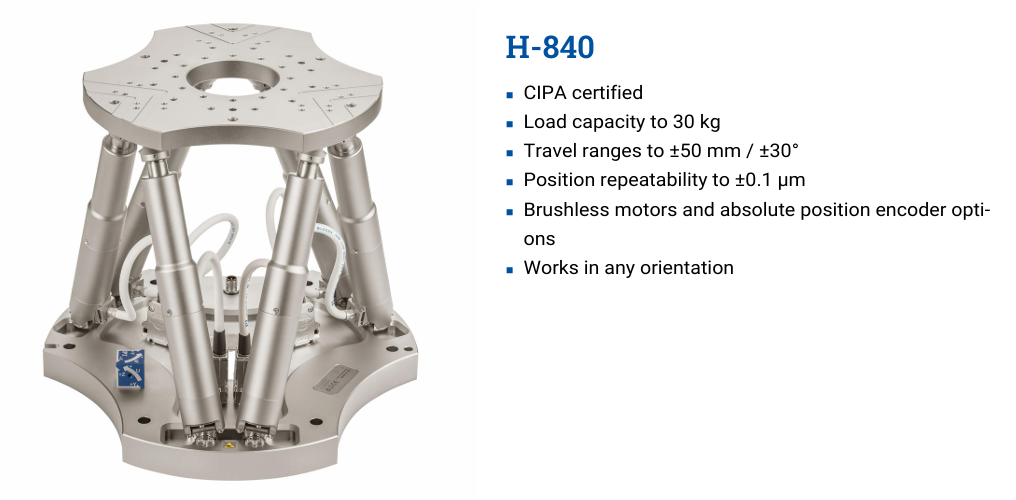
\includegraphics[width=12cm]{imagens/hexapod1.png}

            \textbf{Fonte: } \href{https://www.physikinstrumente.com/fileadmin/user_upload/physik_instrumente/files/datasheets/H-840-Datasheet.pdf}{Physik Instrumente}
            \label{fig:hexapod1}
        \end{figure}
        
        Os principais Hexapods selecionados estão apresentados na \autoref{tab:melhores_hexapods}, a partir das caracteristicas extraídas da tabela geral.  

    \begin{center}
        \centering        
        \scriptsize
        \addtocounter{table}{-1}
        \vspace{-0.3cm}

        {\renewcommand{\arraystretch}{2.2}
        \begin{longtable}{|c|c|c|c|c|}
            \caption{\small Comparação de Hexapods} \label{tab:melhores_hexapods}\\
            \hline
                \fcol{4}{\textbf{Especificação}} & 
                \col{2.6}{\textbf{Physik Instrumente H-840.D2A}} & 
                \col{2.6}{\textbf{Symétrie PUNA}} &
                \col{2.6}{\textbf{Aerotech HEX300-230HL}} & 
                \col{2.6}{\textbf{Moog HX-M300}} \\
            \hline
                \fcol{4}{\textbf{Capacidade de Carga (kg)}} & 
                \col{2.6}{20} & \col{2.6}{150} & \col{2.6}{12} & \col{2.6}{91} \\
            \hline
                \fcol{4}{\textbf{Faixa de Movimento (X/Y/Z mm)}} & 
                \col{2.6}{$\pm 50 / \pm 50 / \pm 25$} & 
                \col{2.6}{$\pm 100 / \pm 100 / \pm 50$} & 
                \col{2.6}{$\pm 55 / \pm 60 / \pm 25$} & 
                \col{2.6}{$\pm 15 / \pm 15 / \pm 10.5$} \\
            \hline
                \fcol{4}{\textbf{Faixa de Rotação (Roll/Pitch/Yaw °)}} & 
                \col{2.6}{$\pm 15 / \pm 15 / \pm 30$} & 
                \col{2.6}{$\pm 23 / \pm 23 / \pm 30$} & 
                \col{2.6}{$\pm 15 / \pm 15 / \pm 30$} & 
                \col{2.6}{$\pm 2.3 / \pm 2.5 / \pm 4.8$} \\
            \hline
                \fcol{4}{\textbf{Precisão (µm)}} & 
                \col{2.6}{0.3 (X/Y/Z)} & \col{2.6}{0.5 (X/Y/Z)} & 
                \col{2.6}{0.015 (X/Y/Z)} & \col{2.6}{1 (X/Y/Z)} \\
            \hline
                \fcol{4}{\textbf{Repetibilidade (µm)}} & 
                \col{2.6}{$\pm 0.3$} & \col{2.6}{$\pm 0.5$} & 
                \col{2.6}{$\pm 0.1$} & \col{2.6}{$\pm 2$} \\
            \hline
                \fcol{4}{\textbf{Tipo de Atuador}} & 
                \col{2.6}{Brushless DC Motor} & 
                \col{2.6}{Brushless Motor with Encoder} & 
                \col{2.6}{Brushless Servomotor} & 
                \col{2.6}{Frameless Torque AC Servo Motor} \\
            \hline
                \fcol{4}{\textbf{Tipo de Sensor}} & 
                \col{2.6}{Absolute Rotary Encoder} & 
                \col{2.6}{Incremental Rotary Encoder} & 
                \col{2.6}{Linear Encoder} & 
                \col{2.6}{Linear Encoder} \\
            \hline
                \fcol{4}{\textbf{Dimensões (mm)}} & 
                \col{2.6}{Ø281 x 189.8} & \col{2.6}{Ø500 x 420} & 
                \col{2.6}{Ø300 x 230} & \col{2.6}{Ø564 x 330} \\
            \hline
                \fcol{4}{\textbf{Comunicação}} & 
                \col{2.6}{Ethernet, USB} & \col{2.6}{Custom} & 
                \col{2.6}{Ethernet, CAN} & \col{2.6}{Custom} \\
            \hline
                \fcol{4}{\textbf{Fonte}} 
                & \col{2.6}{\href{https://tinyurl.com/2c79ve9a}{\textbf{PI}}} 
                & \col{2.6}{\href{https://tinyurl.com/297m8j2p}{\textbf{Symétrie}}} 
                & \col{2.6}{\href{https://tinyurl.com/2ch5pjew}{\textbf{Aerotech}}} 
                & \col{2.6}{\href{https://tinyurl.com/2b4y6pjq}{\textbf{MOOG}}} \\
            \hline
        \end{longtable}}
    
        \small
        \textbf{Fonte:} \href{https://tinyurl.com/2a54wjmx}{Autoria Própria}
    \end{center}
    
    
    \subsection{Atuadores (Pesquisados)}
        Os atuadores DIY para plataformas de movimento 6DOF são amplamente utilizados na construção de simuladores de voo e realidade virtual (VR), permitindo a replicação precisa de deslocamentos e rotações em todas as direções \hyperlink{RAMIREZ}{(RAMIREZ et al., 2012)}. Essas plataformas personalizadas utilizam atuadores lineares ou rotativos, acionados por motores de corrente contínua (DC) ou servos de corrente alternada (AC), proporcionando controle refinado sobre a amplitude de movimento, velocidade e capacidade de carga. 
        A \autoref{fig:atuador} mostra um desses atuadores que poderiam ser utilizados. 
            
        \begin{figure}[H]
            \centering
            \caption{Plataforma Personalizada do Movimento}
            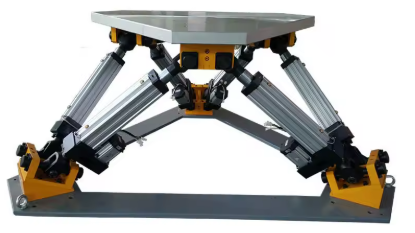
\includegraphics[width=10cm]{imagens/atuador1.png}

            \textbf{Fonte:} \href{https://pt.aliexpress.com/item/1005007512696779.html?spm=a2g0o.detail.pcDetailBottomMoreOtherSeller.1.2d90AX1kAX1k6F&gps-id=pcDetailBottomMoreOtherSeller&scm=1007.40196.417130.0&scm_id=1007.40196.417130.0&scm-url=1007.40196.417130.0&pvid=018e136b-135c-4424-8da8-2a25a8c9cd62&_t=gps-id:pcDetailBottomMoreOtherSeller,scm-url:1007.40196.417130.0,pvid:018e136b-135c-4424-8da8-2a25a8c9cd62,tpp_buckets:668%232846%238109%231935&pdp_npi=4%40dis%21BRL%2119218.99%2119218.99%21%21%2123099.75%2123099.75%21%402101ea8c17391986687045934e6b88%2112000041082239532%21rec%21BR%21%21ABXZ&utparam-url=scene%3ApcDetailBottomMoreOtherSeller%7Cquery_from%3A#nav-store}{AliExpress}
            \label{fig:atuador}
        \end{figure}

        A construção modular dessas estruturas permite ajustes conforme as necessidades específicas da aplicação, tornando-as uma alternativa viável aos sistemas comerciais. Além disso, a precisão dos atuadores é essencial para garantir movimentos suaves e confiáveis, sendo um fator determinante para sua integração em sistemas de monitoramento de movimento. 

    \newpage
    \subsection{Atuadores (Soluções Técnicas)}
        A substituição de Hexapods comerciais por plataformas de movimento personalizadas baseadas em atuadores DIY pode representar uma solução mais econômica e flexível para aplicações industriais e de pesquisa. Ao integrá-las a um Dispositivo de Referência de Monitoramento dos Movimentos (DRMM), torna-se possível simular variações reais de movimento em tempo real, permitindo testes e calibrações mais acessíveis, sendo necessária a calibração e controle da plataforma. Ademais, tais atuadores podem ser aplicados ao projeto, uma vez que é possível transmitir dados em tempo real a partir do MRU para ajustar a movimentação dos atuadores, garantindo que a plataforma replique com precisão as condições dinâmicas de ambientes offshore. A implementação desse sistema pode utilizar protocolos que permitem a transmissão eficiente dos dados captados pelos sensores. Com a fusão de informações provenientes de giroscópios, acelerômetros e magnetômetros, o sistema pode interpretar variações de movimento e calibrar a resposta da plataforma de maneira automática, otimizando a simulação e os testes do DRMM.

        \begin{figure}[H]
            \centering
            \caption{Prototipagem de Simulador de Movimento}
            \frame{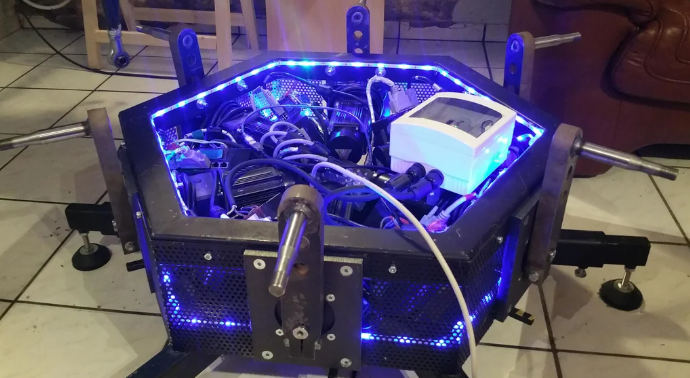
\includegraphics[width=11cm]{imagens/reddit.png}}

            \textbf{Fonte:} \href{https://www.reddit.com/r/flightsim/comments/1djfga0/diy_6dof_motion_simulator_build_for_vr_flight_sims/?show=original&rdt=58142}{Flightsim}
            \label{fig:reeddit}
        \end{figure}

        De acordo com projetos DIY documentados na comunidade r/flightsim (\autoref{fig:reeddit}), a construção de plataformas 6DOF para simuladores de voo exige a integração de atuadores lineares de alta resposta, controladores PID e software dedicado para sincronização dos movimentos. Seguindo essa abordagem, a aplicação desses simuladores no desenvolvimento e calibração do MRU pode permitir a reprodução de movimentos marítimos simulados, validando os sensores do DRMM antes da instalação em navios ou plataformas offshore. Além disso, ao utilizar códigos abertos e controladores acessíveis, como Arduino, ESP32 ou Raspberry Pi, a integração pode ser viabilizada sem a necessidade de investimentos elevados, tornando a solução mais acessível e modular para testes de sensores em diferentes condições operacionais.
        

    \newpage
    \subsection{Definição da Solução Técnica}
        Considerando a abordagem de utilização de atuadores para a simulação de embarcações, um circuito de controle paralelo seria implementado para operar cada pistão de maneira independente, permitindo que o sistema reproduza movimentos complexos definidos por uma equação matemática que descreve a posição da partícula no tempo. Dessa forma, protótipo deve captar esses deslocamentos e validar se as medições correspondem ao comportamento esperado, garantindo que a modelagem matemática do sistema esteja alinhada com os valores experimentais. Para a implementação inicial, um microcontrolador como o ESP32 poderia ser empregado para controlar os atuadores em tempo real utilizando algoritmos PID (Proporcional, Integral, Derivativo). Esse controle permitiria a geração de ondas artificiais que simulam as condições dinâmicas marítimas, sendo essencial para testes de calibração e ajustes do MRU antes de sua aplicação em cenários reais.

        \begin{figure}[H]
            \centering
            \caption{Controle Preditivo Pêndulo Invertido Rotatório}
            \frame{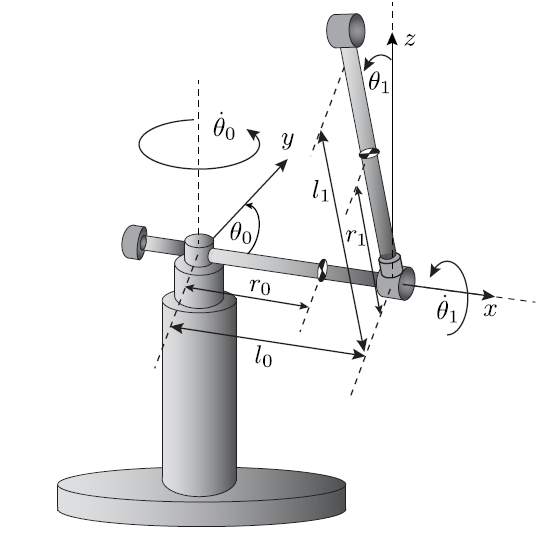
\includegraphics[width=9cm]{imagens/servo.png}}
            
            \textbf{Fonte:} \href{http://scielo.senescyt.gob.ec/scielo.php?script=sci_arttext&pid=S1390-01292020000200049}{Scielo}
            \label{fig:braço}
        \end{figure}

        Alternativamente, servomecanismos poderiam ser incorporados seguindo a mesma lógica de controle, possibilitando a simulação desses movimentos por meio de um braço robótico programável \hyperlink{KOTHARI}{(KOTHARI, 2020)}. Nesse caso, o braço poderia ser modelado para seguir padrões específicos de deslocamento, reproduzindo qualquer trajetória tridimensional predefinida (\autoref{fig:braço}). O sistema de controle determinaria os comandos necessários para que os servomecanismos ajustassem sua posição nos eixos X, Y e Z, permitindo a simulação de diversos tipos de movimentação fluida e dinâmica. Essa abordagem traria flexibilidade adicional ao projeto, possibilitando testes comparativos entre diferentes configurações de sensores e algoritmos para validar a precisão do DRMM em diferentes condições de operação.

    \subsubsection{Comparação de Calibradores}
        A mesma verificação feita para os dispositivos de sensoriamento pode ser implementada de maneira análoga aos atuadores responsáveis pelos movimentos de calibração do sistema. Dessa forma, variáveis como precisão, custo, robustez e durabilidade foram também inseridos para que se possa avaliar qual é a melhor tecnologia a ser utilizada. A \autoref{tab:compcalib} mostra essa comparação pelos critérios abordados.

        \begin{table}[H]
            \centering
            \caption{\small Comparação de Atuadores de Calibração}
            \addtocounter{table}{-1}
            \label{tab:compcalib}
            \vspace{-0.4cm}
            
            \scriptsize
            {\renewcommand{\arraystretch}{2.0}
            \begin{longtable}{|c|c|c|c|}
            \hline
                \fcol{4}{\textbf{Critério}} & 
                \col{3.0}{\textbf{Hexapods}} & 
                \col{3.0}{\textbf{DIY 6 Eixos}} &
                \col{4.0}{\textbf{Braços Robóticos}} \\
            \hline
                \fcol{4}{Precisão} & 
                \col{3.0}{Alta} & 
                \col{3.0}{Baixa a Média} &
                \col{4.0}{Média a Alta (varia conforme modelo e aplicação)} \\
            \hline
                \fcol{4}{Custo} & 
                \col{3.0}{Alto} & 
                \col{3.0}{Baixo a Médio} &
                \col{4.0}{Médio a Alto (industrial) ou Baixo a Médio (educacional/hobby)} \\
            \hline
                \fcol{4}{Nível de Parametrização} & 
                \col{3.0}{Baixo a Médio (controladores dedicados)} & 
                \col{3.0}{Alto (completamente customizável)} &
                \col{4.0}{Médio a Alto (dependendo do sistema de controle e software de programação)} \\
            \hline
                \fcol{4}{Facilidade de Integração} & 
                \col{3.0}{Média (possuem interfaces industriais, mas podem exigir configuração)} & 
                \col{3.0}{Baixa a Média (demandam programação, controladores e eletrônica custom)} &
                \col{4.0}{Média a Alta (robôs industriais costumam ter protocolos de automação bem estabelecidos)} \\
            \hline
                \fcol{4}{Robustez} & 
                \col{3.0}{Alta (uso em ambientes industriais/laboratoriais)} & 
                \col{3.0}{Baixa a Média (depende da fornecedora dos componentes)} &
                \col{4.0}{Média a Alta (robôs industriais são robustos; modelos hobby menos)} \\
            \hline
                \fcol{4}{Durabilidade} & 
                \col{3.0}{Alta} & 
                \col{3.0}{Baixa a Média} &
                \col{4.0}{Média a Alta (varia conforme fabricante e faixa de aplicação)} \\
            \hline
            \end{longtable}}

            \vspace{.15cm}
            \small
            \textbf{Fonte:} Autoria Própria
        \end{table}
        \vspace{-0.2cm}
        
        Uma vez que, diferentemente dos sensores, o escopo do projeto não se baseia no desenvolvimento da construção dos sistemas de atuadores para a calibração, pode ser priorizado um sistema robusto com menor parametrização para agilizar processos de desenvolvimento e alocar a equipe para tarefas com maior demanda no que se refere ao protótipo a ser construído. Dessa forma, será priorizado os dispositivos robustos e com alta confiabilidade de mercado.
        
    \newpage

\newpage
\section{Metodologia de Execução}
    Para a realização do projeto, definiu-se um esquema de organização que divide as tarefas em equipes especializadas, cada qual responsável por uma etapa específica. Enquanto uma unidade se empenha na pesquisa e seleção dos sensores adequados, outra se ocupa da elaboração de hardware e firmware, existindo ainda um grupo dedicado ao desenvolvimento do software de comunicação e à realização dos testes de validação. Esse procedimento permite que cada componente do sistema seja planejado e verificado de forma independente, resultando em uma integração final mais segura e eficiente.

    Para manter as equipes em sintonia e assegurar que as metas sejam cumpridas, foram instituídas reuniões semanais. Nesses encontros, cada grupo apresenta seus avanços, avalia-se o estágio geral do projeto e discutem-se possíveis entraves técnicos. As informações coletadas são então confrontadas com os parâmetros estabelecidos no planejamento, o que possibilita a adoção de ajustes imediatos e a correção de rotas, sempre que necessário. Além disso, essa dinâmica otimiza o uso de recursos, evitando despesas supérfluas e concentrando esforços nas soluções mais promissoras.
    
    Quando cada ciclo de trabalho é finalizado, todos os dados reunidos são organizados em um relatório técnico. Esse documento oferece uma visão precisa do ponto em que o projeto se encontra, indica desafios pendentes e orienta as próximas etapas a serem seguidas. A manutenção constante dessa documentação torna mais claro o histórico de escolhas feitas, contribui para uma coordenação de projeto mais eficiente e assegura o cumprimento das principais entregas dentro dos prazos estipulados.

\newpage
\section{Conclusão}
    De acordo com os dados supracitados, a Macroentrega 1 do projeto tem como foco a pesquisa e seleção de dispositivos de referência de movimento (MRUs), módulos inerciais (IMUs) e sensores, visando o desenvolvimento de uma solução nacional para monitoramento de movimentos em ambientes offshore. Para isso, foram analisadas as características técnicas de diferentes modelos comerciais, considerando precisão, confiabilidade e compatibilidade com as necessidades do setor. Além da seleção dos dispositivos, foram definidas estratégias de calibração e validação do desempenho em condições reais, utilizando plataformas de testes dinâmicos. Esse processo busca garantir a eficiência e a robustez do sistema, assegurando que o dispositivo desenvolvido atenda aos padrões exigidos pela indústria.

    A solução técnica foi estruturada em três frentes de trabalho, distribuídas entre equipes especializadas. A primeira equipe ficou responsável pelo desenvolvimento e integração dos sensores, a segunda concentrou-se nos módulos IMU e MRU, enquanto a terceira equipe dedicou-se ao desenvolvimento do software de processamento e comunicação dos dados. A aquisição dos dispositivos selecionados permitirá a realização de testes experimentais, avaliando a possibilidade de otimização da precisão por meio de algoritmos avançados, como redes neurais e ajuste de funções multivariáveis. Com essa abordagem, o projeto não apenas busca reduzir a dependência de equipamentos importados, mas também promover autonomia tecnológica e inovação no setor offshore.
    

    \newpage
    \newpage

% ATIVA O CABEÇALHO DAS REFERÊNCIAS
\pagestyle{modeloReferencias}

% ADICIONA UM TIPO "SECTION" CUSTOMIZADO NO SUMÁRIO
\addcontentsline{toc}{section}{REFERÊNCIAS}

% CRIA UMA SECTION SEM NUMERAÇÃO
\section*{REFERÊNCIAS}
\vspace{-1cm}

\referencia
    {ELECTRONOOBS}
    {Tutorial Arduino MPU6050 IMU}
    {2018}
    {\url{https://electronoobs.com/eng_arduino_tut76.php}}
    {24 fev. 2025}

\referencia
    {EMBARCADOS}
    {IMUs - Unidades de Medicao Inercial}
    {2019}
    {\url{https://embarcados.com.br/imus-unidades-de-medicao-inercial/}}
    {18 fev. 2025}

\referencia
    {FM2S}
    {Tipos de riscos na logistica}
    {2015}
    {\url{https://www.fm2s.com.br/blog/tipos-de-riscos-na-logistica}}
    {24 fev. 2025}

\referencia
    {KOTHARI}
    {Six Degree of Freedom Robotic Arm with Mimicking Mechanism}
    {2020}
    {\url{https://arxiv.org/abs/2012.14286}}
    {12 fev. 2025}

\referencia
    {MACARIO}
    {Utilização de Filtros Adaptativos para Detecção de Falhas em Mancais de Rolamentos}
    {2006}
    {\url{https://repositorio.ufu.br/handle/123456789/15039}}
    {12 fev. 2025}

\referencia
    {MARINHA}
    {Normas da Autoridade Maritima para Homologacao de Helideques Instalados em Embarcacoes e Plataformas Maritimas}
    {2017}
    {\url{https://www.marinha.mil.br/dpc/sites/www.marinha.mil.br.dpc/files/normam27.pdf}}
    {18 fev. 2025}

\referencia
    {MORAES}
    {Caracterizacao de Sensores Inerciais do Tipo MEMS para Medicao Direcional de Ondas}
    {2015}
    {\url{https://tinyurl.com/27kog7sm}}
    {05 fev. 2025}

\referencia
    {ORTIZ NETO}
    {Trajetorias tecnologicas no segmento offshore: ambiente e oportunidades}
    {2008}
    {\url{https://www.scielo.br/j/rec/a/Y5bP5b6BYGzW3qrtzdfcxdC/}}
    {18 fev. 2025}

\referencia
    {PI}
    {Hexapods: Motion Platforms with Six Degrees of Freedom}
    {2025}
    {\url{https://www.physikinstrumente.com/en/products/hexapods/}}
    {18 fev. 2025}

\referencia
    {RAMIREZ}
    {Automacao de Plataforma de Movimentos 6 DOF para Simulador de Voo em Realidade Virtual Imersiva}
    {2012}
    {\url{https://www.revistas.udesc.br/index.php/hfd/article/view/2880}}
    {18 fev. 2025}

\referencia
    {RONCETTI}
    {Elaboracao de diagramas de limite operacional para procedimentos de icamento offshore}
    {2014}
    {\url{https://tinyurl.com/2dhtuyld}}
    {05 fev. 2025}

\referencia
    {SHIPMOTION}
    {SMC manufactures motion reference units for the Marine and Offshore Oil and Gas industry}
    {2024}
    {\url{https://www.shipmotion.eu/}}
    {18 fev. 2025}

\referencia
    {UNICAMP}
    {Calibracao de Sensores Inerciais}
    {2021}
    {\url{https://tecnologias.inova.unicamp.br/tecnologia/1156_inerciais/}}
    {03 fev. 2025}

\phantom{a}

\end{document}